\chapter{Sterile Neutrino Oscillation Inputs Within SBN}
\label{chap:osc_inputs}


\begin{figure}[!h]
    \centering
    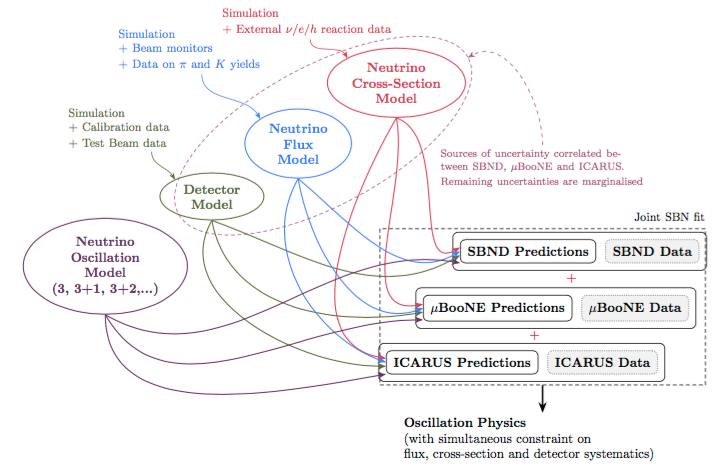
\includegraphics[width = \largefigwidth]{figures-chap5/valor_analysis.png}
    \caption{Overview of the SBN oscillation analysis paradigm. A given model for the neutrino oscillation, detector, neutrino flux and neutrino cross-section are combined with the appropriate data to give the prediction for the respective detector. Individual detector predictions may be combined to give an overall \gls{sbn} prediction. }
    \label{fig:analysis_paradigm}
\end{figure}

\section{Event Production}


\subsection{\texorpdfstring{\numu}{numu}}
\subsection{\texorpdfstring{\nue}{nue}}
The $\nue $ production followed the same steps described in section \ref{S:MCSamples:NumuProd}, however, in addition to generating an intrinsic $\nue$ sample, an oscillated $\numu \rightarrow \nue$ sample, a dirt sample and a cosmic sample were also produced. The oscillated sample is used to mimic the $\nue$ appearance signal whereas the dirt and cosmic samples are backgrounds. The other major background associated with a $\nue$ analysis involves $\numu$. A dedicated sample was not produced to emulate this, but instead the events from the $\numu$ production were also ran through the $\nue$ selection as mentioned in section \ref{S:NuESelection}. Table \ref{T:nue_production} outlines the number of events produced for each sample for each detector. The dirt events were produced with an additional filter at the generation stage which discarded any events where a shower above 10 MeV in the active volume was not present. This filter was used in order to remove any delta rays. Only about 1\% of dirt events would pass this filter so the number of dirt events used in the $\nue$ selection was $\sim$100,000. 


\begin{table}[h!]
\begin{tabular}{c cc}
Sample        & \begin{tabular}[c]{@{}c@{}}Events Produced\end{tabular} \\ \hline

Intrinsic $\nue$ & $\sim$1,000,000      \\
Oscillated $\nu$ & $\sim$1,000,000      \\
$\numu$          & {See $\nu_{\mu}$ sample}  \\
Dirt          & $\sim$10,000,000        \\
Cosmic\_Dirt  & $\sim$100,000             

\end{tabular}
\caption{The number of events initially produced for each sample in each of the three SBN detectors as part of the $\nue$ analysis.}
\end{table}\label{T:nue_production}


\section{\texorpdfstring{$\nu_\mu$ and $\nu_e$ Selections}{numu and nue Selections}}
Link in with Energy Reco. section

\section{Reaction Modes}
\subsection{Fine}

% Fine reaction modes
\begin{table}[t!]
  \renewcommand{\arraystretch}{1.6}
  \begin{tabular}{>{\centering\arraybackslash}m{4cm} 
                  >{\centering\arraybackslash}m{4cm}
                  >{\centering\arraybackslash}m{4cm}}
  
    \toprule
    \multicolumn{3}{c}{\textit{Fine Reaction Modes}} \\
    $\numu$, $\numubar$ & $\nue$, $\nuebar$ & $\numu \rightarrow \nue, \numubar \rightarrow \nuebar$ \\
    \midrule
    CC QE                      & CC QE                     & CC QE\\
    NC~Elastic                 & NC~Elastic                & CC MEC\\ 
    CC, NC MEC                 & CC, NC MEC                & CC 1$\pi^{\pm}$ \\  
    CC, NC 1$\pi^{\pm}$        & CC, NC 1$\pi^{\pm}$       & CC 1$\pi^{0}$ \\   
    CC, NC 1$\pi^{0}$          & CC, NC 1$\pi^{0}$         & CC 2$\pi^{\pm}$ \\   
    CC, NC 2$\pi^{\pm}$        & CC, NC 2$\pi^{\pm}$       & CC 2$\pi^{0}$i \\   
    CC, NC 2$\pi^{0}$          & CC, NC 2$\pi^{0}$         & CC Coh \\   
    CC, NC $\pi^{\pm}\pi^{0}$  & CC, NC $\pi^{\pm}\pi^{0}$ & Elastic Scattering \\   
    CC, NC Coh                 & CC, NC Coh                & CC Other \\  
    CC, NC Elastic Scattering  & CC+NC Elastic Scattering  \\  
    NC 1$\gamma$               & NC 1$\gamma$              \\  
    CC, NC Other               & CC, NC Other              \\  
    \hdashline
    \multicolumn{3}{c}{\textit{Cosmic \& Dirt}} \\
    \bottomrule

  \end{tabular}
  \caption[Fine Reaction Modes]{The complete list of reaction modes considered in an \gls{sbn} analysis.}
  \label{table:fine_reac_modes}
\end{table}




\subsection{Coarse}
% Coarse reaction modes
\begin{table}[t!]
  \begin{tabular}{>{\centering\arraybackslash}m{4cm} 
    >{\centering\arraybackslash}m{4cm}}
  
    \toprule
    \multicolumn{2}{c}{\textit{Coarse Reaction Modes}} \\
    $\numu$, $\numubar$ & $\nue$, $\nuebar$ \\
    \midrule
    $\numu$ CC QE          & \nue CC QE          \\ 
    $\numu$ CC MEC         & \nue CC MEC         \\ 
    $\numu$ CC 1$\pi$      & \nue CC 1$\pi$      \\ 
    $\numu$ CC 2$\pi$      & \nue CC 2$\pi$      \\ 
    $\numu$ CC Other       & \nue CC Other       \\ 
    $\numubar$ CC          & \nuebar CC          \\
    $\nue$ \& $\nuebar$ CC & \numu CC            \\
    NC                     & \numubar CC         \\
    \textit{Cosmic}        & Oscillated \nue CC  \\
    \textit{Dirt}          & NC 0\pi             \\
                           & NC Other            \\
                           & \textit{Cosmic}     \\
                           & \textit{Dirt}       \\
    \bottomrule

  \end{tabular}
  \caption[Coarse Reaction Modes]{The \textit{coarse} reaction modes used for both the \numu and \nue channels. These are broader definition of the reaction modes where one or more of the \textit{fine} reaction modes listed in \TableRef{table:fine_reac_modes} would come under the umbrella of a given coarse reaction mode.}
  \label{table:coarse_reac_modes}
\end{table}


\section{Flux Systematics}

\begin{table}[!h]
  \renewcommand{\arraystretch}{1.4}    
  \begin{tabular}{p{2.5cm} p{9.2cm} p{1.2cm} p{1.2cm}}
    \toprule
    \multirow{2}{*}{Parameter} & \multirow{2}{*}{Description} & \multicolumn{2}{c}{Uncertainty} \\
    && \multicolumn{1}{c}{Be} & \multicolumn{1}{c}{Al} \\
    \midrule

    $f_{\sigma_{INEL}^{N}}$   & Secondary inelastic nucleon cross-section in the target (Be) and horn (Al) & $\pm 5 \%$ & $\pm 10 \%$\\
                            
    $f_{\sigma_{QE}^{N}}$     & Secondary quasi-elastic nucleon cross-section in the target (Be) and horn (Al) & $\pm 20 \%$ & $\pm 45 \%$\\
                            
    $f_{\sigma_{TOT}^{N}}$    & Secondary total nucleon cross-section in the target (Be) and horn (Al) & $\pm 15 \%$ & $\pm 25 \%$\\

    $f_{\sigma_{INEL}^{\pi}}$ & Secondary inelastic pion cross-section in the target (Be) and horn (Al) & $\pm 10 \% $ & $\pm 20 \% $\\
                          
    $f_{\sigma_{QE}^{\pi}}$   & Secondary quasi-elastic pion cross-section in the target (Be) and horn (Al) & $\pm 11.2 \% $ & $\pm 25.9 \% $\\
                          
    $f_{\sigma_{TOT}^{\pi}}$  & Secondary total pion cross-section in the target (Be) and horn (Al) & $\pm 11.9 \%$ & $\pm 28.7 \%$\\
    \bottomrule
  \end{tabular}
  \caption[Hadronic secondary interaction flux systematic parameters]{The systematic uncertainties associated with secondary hadron interaction cross-sections in both the horn (Aluminium) and the target (Berylium) \cite{SBN_Proposal}}.
  \label{}
\end{table}


\begin{table}[!h]
  \renewcommand{\arraystretch}{1.4}    
  \begin{tabular}{p{2.5cm} p{10cm} p{2cm}}

    \toprule
    Parameter & Description & Uncertainty \\ 
    \midrule

    $f_{SkinEffect}$  & Depth that the current penetrates the horn conductor & $<18 \%$\\

    $f_{HornCurrent}$ & Current running in the horn conductor & $\pm 0.6 \%$\\
    \bottomrule

  \end{tabular}
  \caption[Optical, beam focusing flux systematic parameters]{Optical systematic flux uncertainties associated with the current in the horn\cite{BNB_flux}.}
  \label{}
\end{table}

\begin{table}[!h]
  \renewcommand{\arraystretch}{1.4}    
  \begin{tabular}{p{2cm} p{6.0cm} p{1.2cm} p{1.2cm} p{1.2cm} p{1.2cm}}
    \toprule
    \multirow{2}{*}{Parameter} & \multirow{2}{*}{Description} & \multicolumn{4}{c}{Uncertainty} \\
    && \multicolumn{1}{c}{$\nu_{\mu}$} & \multicolumn{1}{c}{$\bar{\nu}_{\mu}$} & \multicolumn{1}{c}{$\nu_{e}$} & \multicolumn{1}{c}{$\bar{\nu}_{e}$} \\
    \midrule

    $f_{\pi^{+}}$ & $\nu$ production mechanism: $\pi^{+}$ & $ \pm 11.7 \%$ & $ \pm 1.0 \%$ & $ \pm 10.7 \%$ & $ \pm 0.03 \%$ \\

    $f_{\pi^{-}}$ & $\nu$ production mechanism: $\pi^{-}$ & $ \pm 0.0 \%$ & $ \pm 11.6 \%$ & $ \pm 0.0 \%$ & $ \pm 3.0 \%$ \\

    $f_{K^{+}}$   & $\nu$ production mechanism: $K^{+}$ & $ \pm 0.2 \%$ & $ \pm 0.1 \%$ & $ \pm 2.0 \%$ & $ \pm 0.1 \%$ \\
                  
    $f_{K^{-}}$   & $\nu$ production mechanism: $K^{-}$ & $ \pm 0.0 \%$ & $ \pm 0.4 \%$ & $ \pm 0.0 \%$ & $ \pm 3.0 \%$ \\
                  
    $f_{K^{0}}$   & $\nu$ production mechanism: $K^{0}$ & $ \pm 0.0 \%$ & $ \pm 0.3 \%$ & $ \pm 2.3 \%$ & $ \pm 21.4 \%$ \\

    \bottomrule
  \end{tabular}
  \caption[Hadron production flux systematic parameters]{Hadron production systematic flux uncertainties \cite{BNB_flux_TN}.}
  \label{}
\end{table}

\begin{figure}
    \centering
    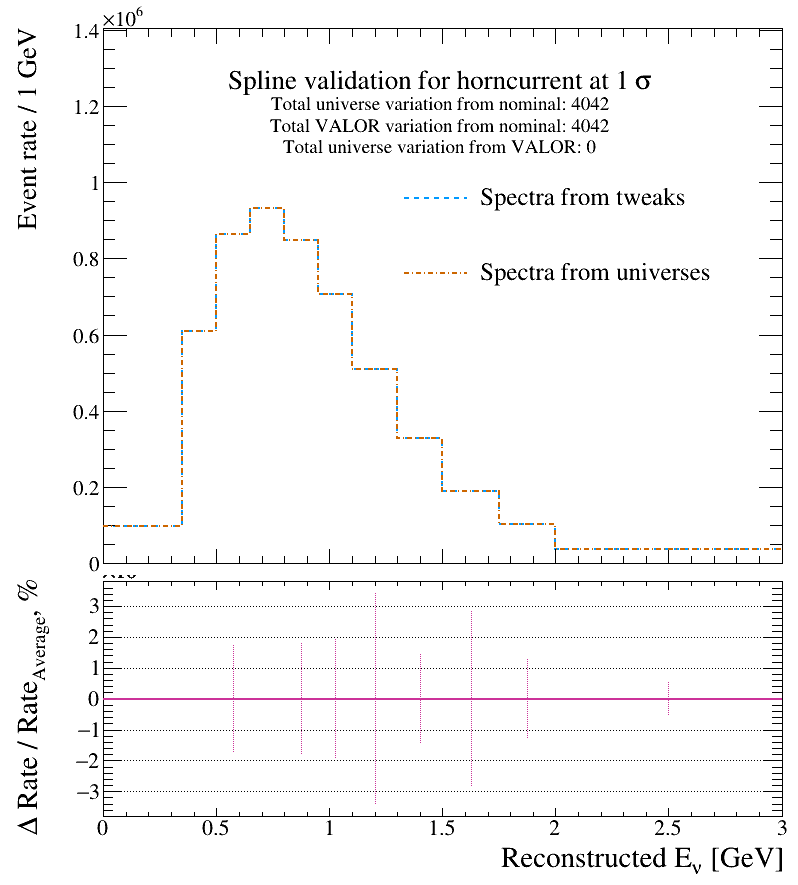
\includegraphics[width = \largefigwidth]{figures-chap5/tweak_nsigma_nue/horncurrent_FluxUnisim_nuelikeCChigh_1sigma_horncurrent_FluxUnisim.png}
    \caption[+1$\sigma$ variation comparison for the horncurrent\_FluxUnisim parameter.]{A comparison of the +1$\sigma$ variation from the response functions in VALOR and the universes for the 'horncurrent\_FluxUnisim' flux systematic parameter.}
    \label{fig:my_label}
\end{figure}

\begin{figure}
    \centering
    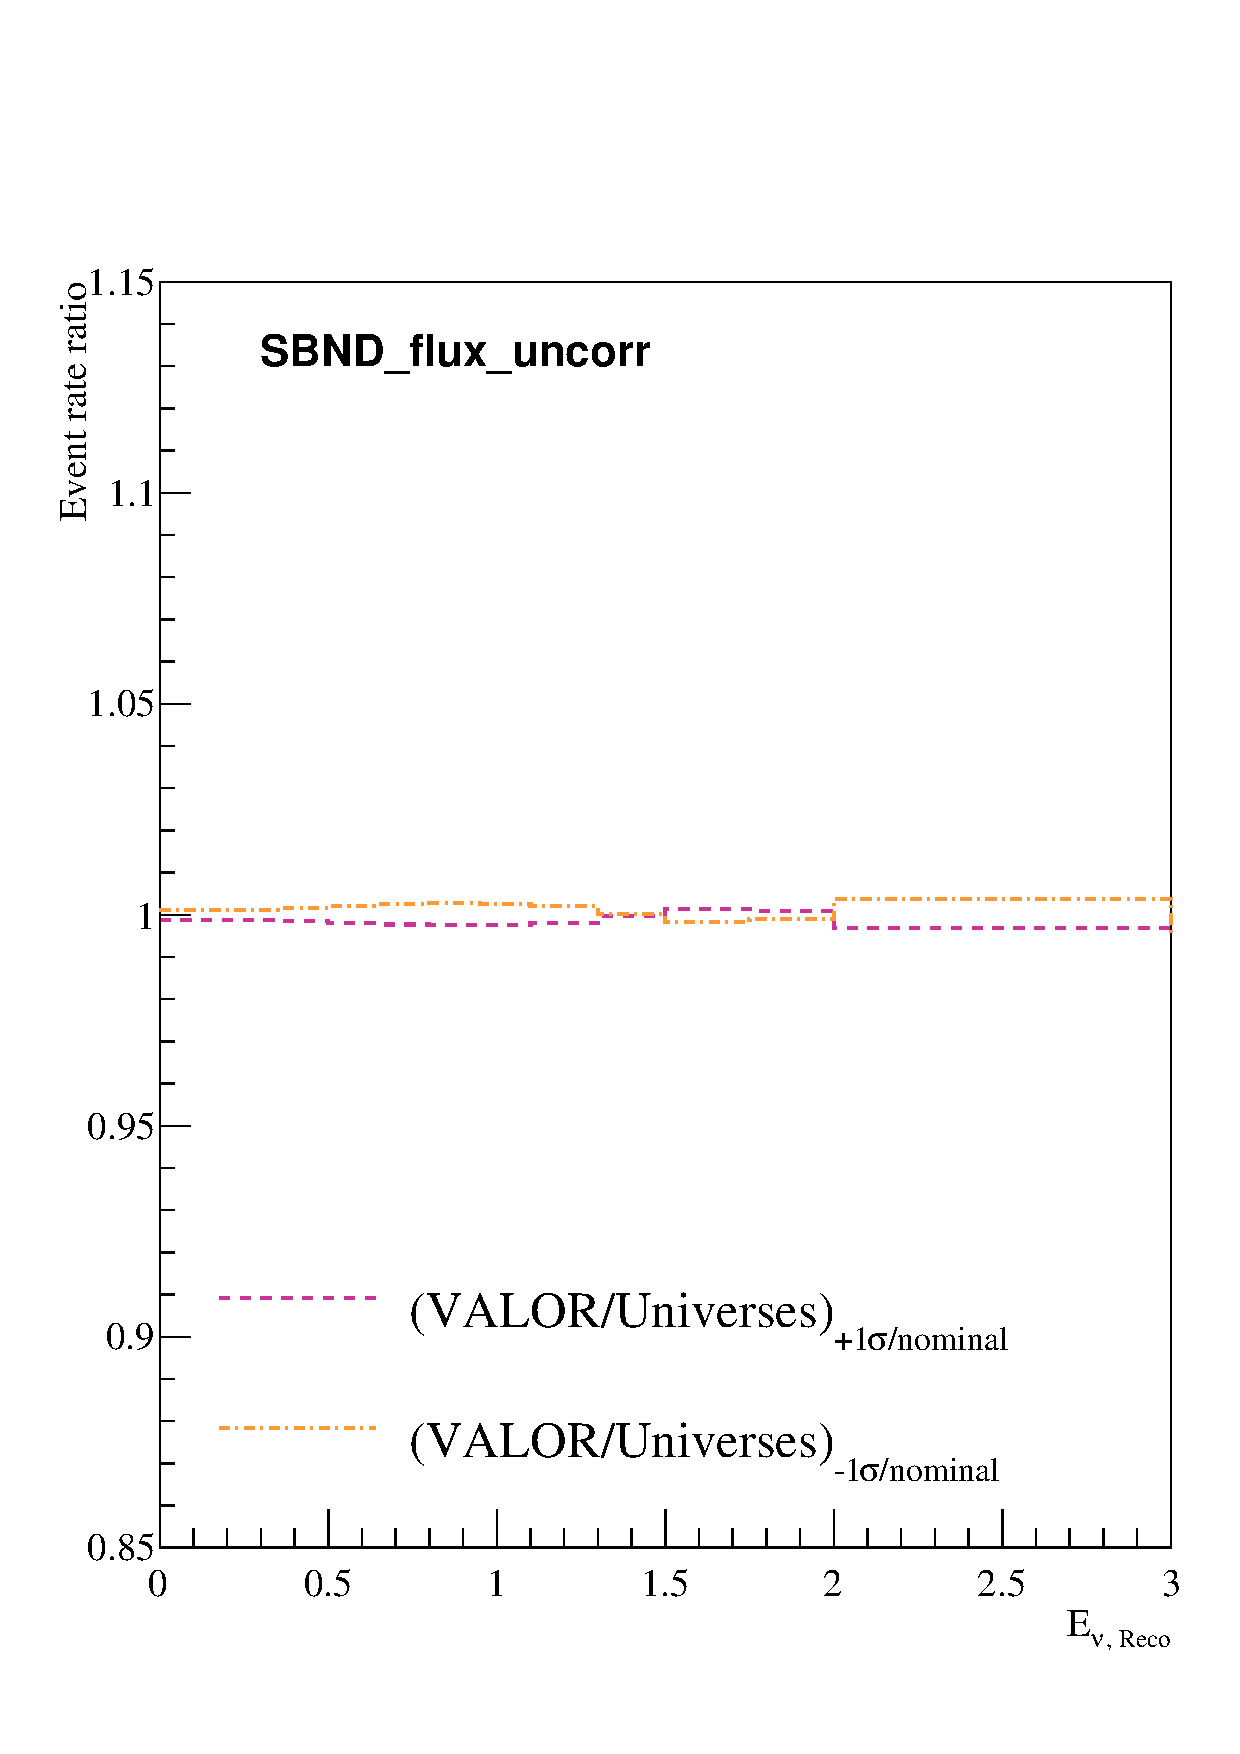
\includegraphics[width = \largefigwidth]{figures-chap5/tweak_pdf_N_nue/universe_valor_double_ratios_SBND_flux_uncorr.pdf}
    \caption{Caption}
    \label{fig:my_label}
\end{figure}

\section{Interaction Systematics}

\begin{table}[h!]
    \renewcommand{\arraystretch}{1.4}
    \begin{tabular}{p{1.8cm} p{10cm}>{\centering\arraybackslash}p{ 2.2cm}}
        \toprule
         Parameter & Description & $\delta P / P$ \\
        \midrule
         $f_{M_{A}^{CCQE}}$  & Axial mass for CC quasi-elastic & -15\% +25\% \\
         
         $f_{M_{A}^{CCRes}}$ & Axial mass for CC resonance neutrino production & $\pm 20\%$ \\
         
         $f_{M_{A}^{NCRes}}$ & Axial mass for NC resonance neutrino production & $\pm 20\%$ \\
         
         $f_{NC}$              & Additional error on NC/CC ratio & $\pm 25\%$ \\
         
         $f_{nR_{\nu n}^{CC1\pi}}$ & Non-resonance bkg normalisation in $\nu n$ CC1$\pi$ reactions & $\pm 50\%$ \\
         
         $f_{nR_{\nu p}^{CC1\pi}}$ & Non-resonance bkg normalisation in $\nu p$ CC1$\pi$ reactions & $\pm 50\%$ \\
         
         $f_{nR_{\nu n}^{CC2\pi}}$ & Non-resonance bkg normalisation in $\nu n$ CC2$\pi$ reactions & $\pm 50\%$ \\
         
         $f_{nR_{\nu p}^{CC2\pi}}$ & Non-resonance bkg normalisation in $\nu p$ CC2$\pi$ reactions & $\pm 50\%$ \\
         
         $f_{nR_{\bar{\nu} n}^{CC1\pi}}$ & Non-resonance bkg normalisation in $\bar{\nu} n$ CC1$\pi$ reactions & $\pm 50\%$ \\
         
         $f_{nR_{\bar{\nu} p}^{CC1\pi}}$ & Non-resonance bkg normalisation in $\bar{\nu} p$ CC1$\pi$ reactions & $\pm 50\%$ \\
         
         $f_{nR_{\bar{\nu} n}^{CC2\pi}}$ & Non-resonance bkg normalisation in $\bar{\nu} n$ CC2$\pi$ reactions & $\pm 50\%$ \\
         
         $f_{nR_{\bar{\nu} p}^{CC2\pi}}$ & Non-resonance bkg normalisation in $\bar{\nu} p$ CC2$\pi$ reactions & $\pm 50\%$ \\
        
         $f_{nR_{\nu n}^{NC1\pi}}$ & Non-resonance bkg normalisation in $\nu n$ NC1$\pi$ reactions & $\pm 50\%$ \\
         
         $f_{nR_{\nu p}^{NC1\pi}}$ & Non-resonance bkg normalisation in $\nu p$ NC1$\pi$ reactions & $\pm 50\%$ \\
         
         $f_{nR_{\nu n}^{NC2\pi}}$ & Non-resonance bkg normalisation in $\nu n$ NC2$\pi$ reactions & $\pm 50\%$ \\
         
         $f_{nR_{\nu p}^{NC2\pi}}$ & Non-resonance bkg normalisation in $\nu p$ NC2$\pi$ reactions & $\pm 50\%$ \\
         
         $f_{nR_{\bar{\nu} n}^{NC1\pi}}$ & Non-resonance bkg normalisation in $\bar{\nu} n$ NC1$\pi$ reactions & $\pm 50\%$ \\
         
         $f_{nR_{\bar{\nu} p}^{NC1\pi}}$ & Non-resonance bkg normalisation in $\bar{\nu} p$ NC1$\pi$ reactions & $\pm 50\%$ \\
         
         $f_{nR_{\bar{\nu} n}^{NC2\pi}}$ & Non-resonance bkg normalisation in $\bar{\nu} n$ NC2$\pi$ reactions & $\pm 50\%$ \\
         
         $f_{nR_{\bar{\nu} p}^{NC2\pi}}$ & Non-resonance bkg normalisation in $\bar{\nu} p$ NC2$\pi$ reactions & $\pm 50\%$ \\
        
        \bottomrule
        
    \end{tabular}
    \caption[SBN proposal interaction cross-section systematic parameters]{GENIE interaction cross-section systematics considered in \gls{sbn} as part of the \textit{proposal} set of systematics. \cite{GENIE_manual}.}
    \label{}
\end{table}


\begin{table}[h!]
    \renewcommand{\arraystretch}{1.4}
    \begin{tabular}{p{1.8cm} p{10cm}>{\centering\arraybackslash}p{ 2.2cm}}
        \toprule
         Parameter & Description & $\delta P / P$ \\
        \midrule
         $f_{M_{A}^{NCEl}}$  & Axial mass for NC elastic & $\pm 25\%$ \\
         
         $f_{\eta^{NCEl}}$    & Strange axial form factor for NC elastic & $\pm 30\%$ \\
        
         %$f_{2p2h}$          & Normalisation uncertainty for 2p2h interactions & $\pm 100\%$ \\
         
         $f_{M_{V}^{CCRes}}$ & Vector mass for CC resonance neutrino production & $\pm 10\%$ \\
         
         $f_{M_{V}^{NCRes}}$ & Vector mass for NC resonance neutrino production & $\pm 10\%$ \\
         
         $f_{A_{HT}}$          & Higher-twist parameter A for NC and CC DIS events & $\pm 25\%$ \\
         
         $f_{B_{HT}}$          & Higher-twist parameter B for NC and CC DIS events & $\pm 25\%$ \\
         
         $f_{C_{v1u}}$         & Valence p.d.f. correction factor $C_{v1u}$ for DIS events & $\pm 30\%$ \\
         
         $f_{C_{v2u}}$         & Valence p.d.f. correction factor $C_{v2u}$ for DIS events & $\pm 40\%$ \\
         
         $f_{M_{A}^{Coh}}$     & Axial mass for NC and CC coherent pion production & $ \pm 50 \%$ \\
         
         $f_{R_{0}^{Coh}}$     & Nuclear size parameter controlling $\pi$ absorption & $\pm 20 \%$ \\
        
        $f_{\Delta\rightarrow N\gamma}$   & Branching ratio for $\Delta$ radiative decay & $\pm 50 \%$ \\
        
        \bottomrule
        
    \end{tabular}
    \caption[Modern interaction cross-section systematic parameters]{GENIE interaction cross-section systematics considered in \gls{sbn} as part of the \textit{modern} set of systematics \cite{GENIE_manual}.}

    \label{}
\end{table}


\begin{table}[!h]
    \renewcommand{\arraystretch}{1.4}
    \begin{tabular}{p{1.8cm} p{11.4cm} p{1.2cm}}
        \toprule
         Parameter & Description & $\delta P / P$ \\
        \midrule
        
         $f_{\lambda_{\pi}}$   & Intranuclear mean free path for pions & $ \pm 20 \% $ \\
        
         $f_{R^{CEx}_{\pi}}$    & Intranuclear charge exchange rescattering fraction for pions & $ \pm 50 \% $ \\
        
         $f_{R^{Inel}_{\pi}}$   & Intranuclear inelastic rescattering fraction for pions & $ \pm 40 \% $ \\
        
         $f_{R^{\pi}_{\pi}}$    & Intranuclear pion-production rescattering fraction for pions & $ \pm 20 \% $ \\
        
         $f_{R^{Abs}_{\pi}}$    & Intranuclear absorption fraction for pions & $ \pm 20 \% $ \\
        
         $f_{\lambda_{N}}$     & Intranuclear mean free path for nucleons & $ \pm 20 \% $ \\
        
         $f_{R^{CEx}_{N}}$      & Intranuclear charge exchange rescattering fraction for nucleons & $ \pm 50 \%$ \\
        
         $f_{R^{Inel}_{N}}$     & Intranuclear inelastic rescattering fraction for nucleons & $ \pm 40 \% $ \\
        
         $f_{R^{\pi}_{N}}$      & Intranuclear pion-production rescattering fraction for nucleons & $ \pm 20 \% $ \\
        
         $f_{R^{Abs}_{N}}$      & Intranuclear absorption fraction for nucleons & $ \pm 20 \% $ \\

        \bottomrule
    \end{tabular}
    \caption[Intranuclear hadron transport systematic parameters]{\cite{GENIE_manual}}
    \label{}
\end{table}

\begin{figure}
    \centering
    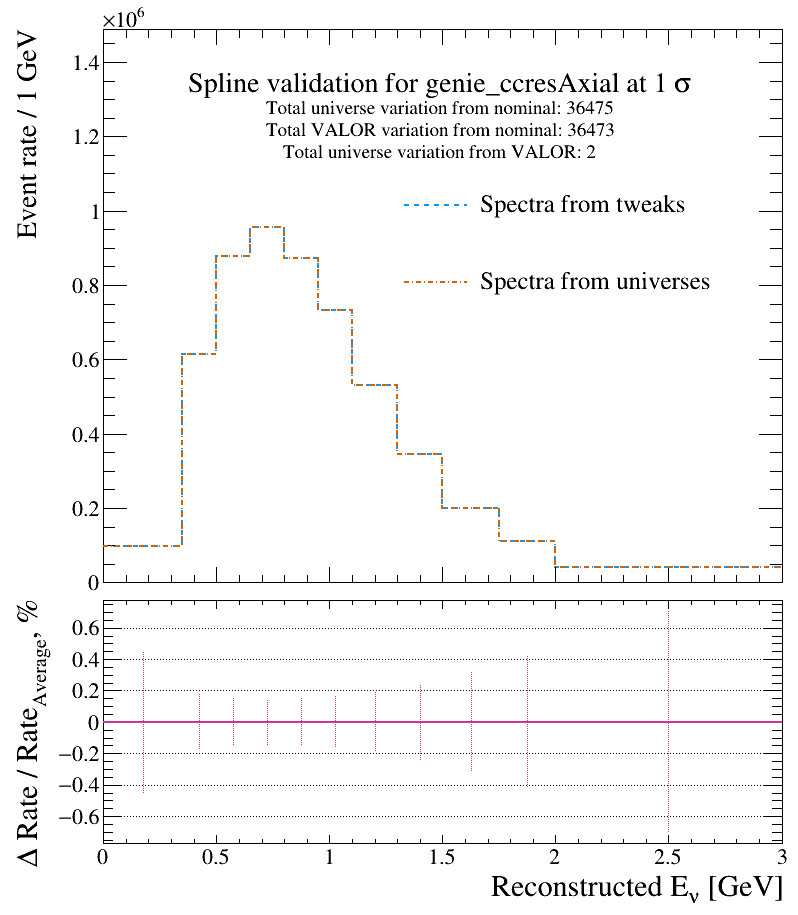
\includegraphics[width = \largefigwidth]{figures-chap5/tweak_nsigma_nue/genie_ccresAxial_Genie_nuelikeCChigh_1sigma_genie_ccresAxial_Genie.png}
    \caption[+1$\sigma$ variation comparison for the genie\_ccresAxial\_Genie parameter.]{A comparison of the +1$\sigma$ variation from the response functions in VALOR and the universes for the 'genie\_ccresAxial\_Genie' proposal interaction systematic parameter.}
    \label{fig:my_label}
\end{figure}

\begin{figure}
    \centering
    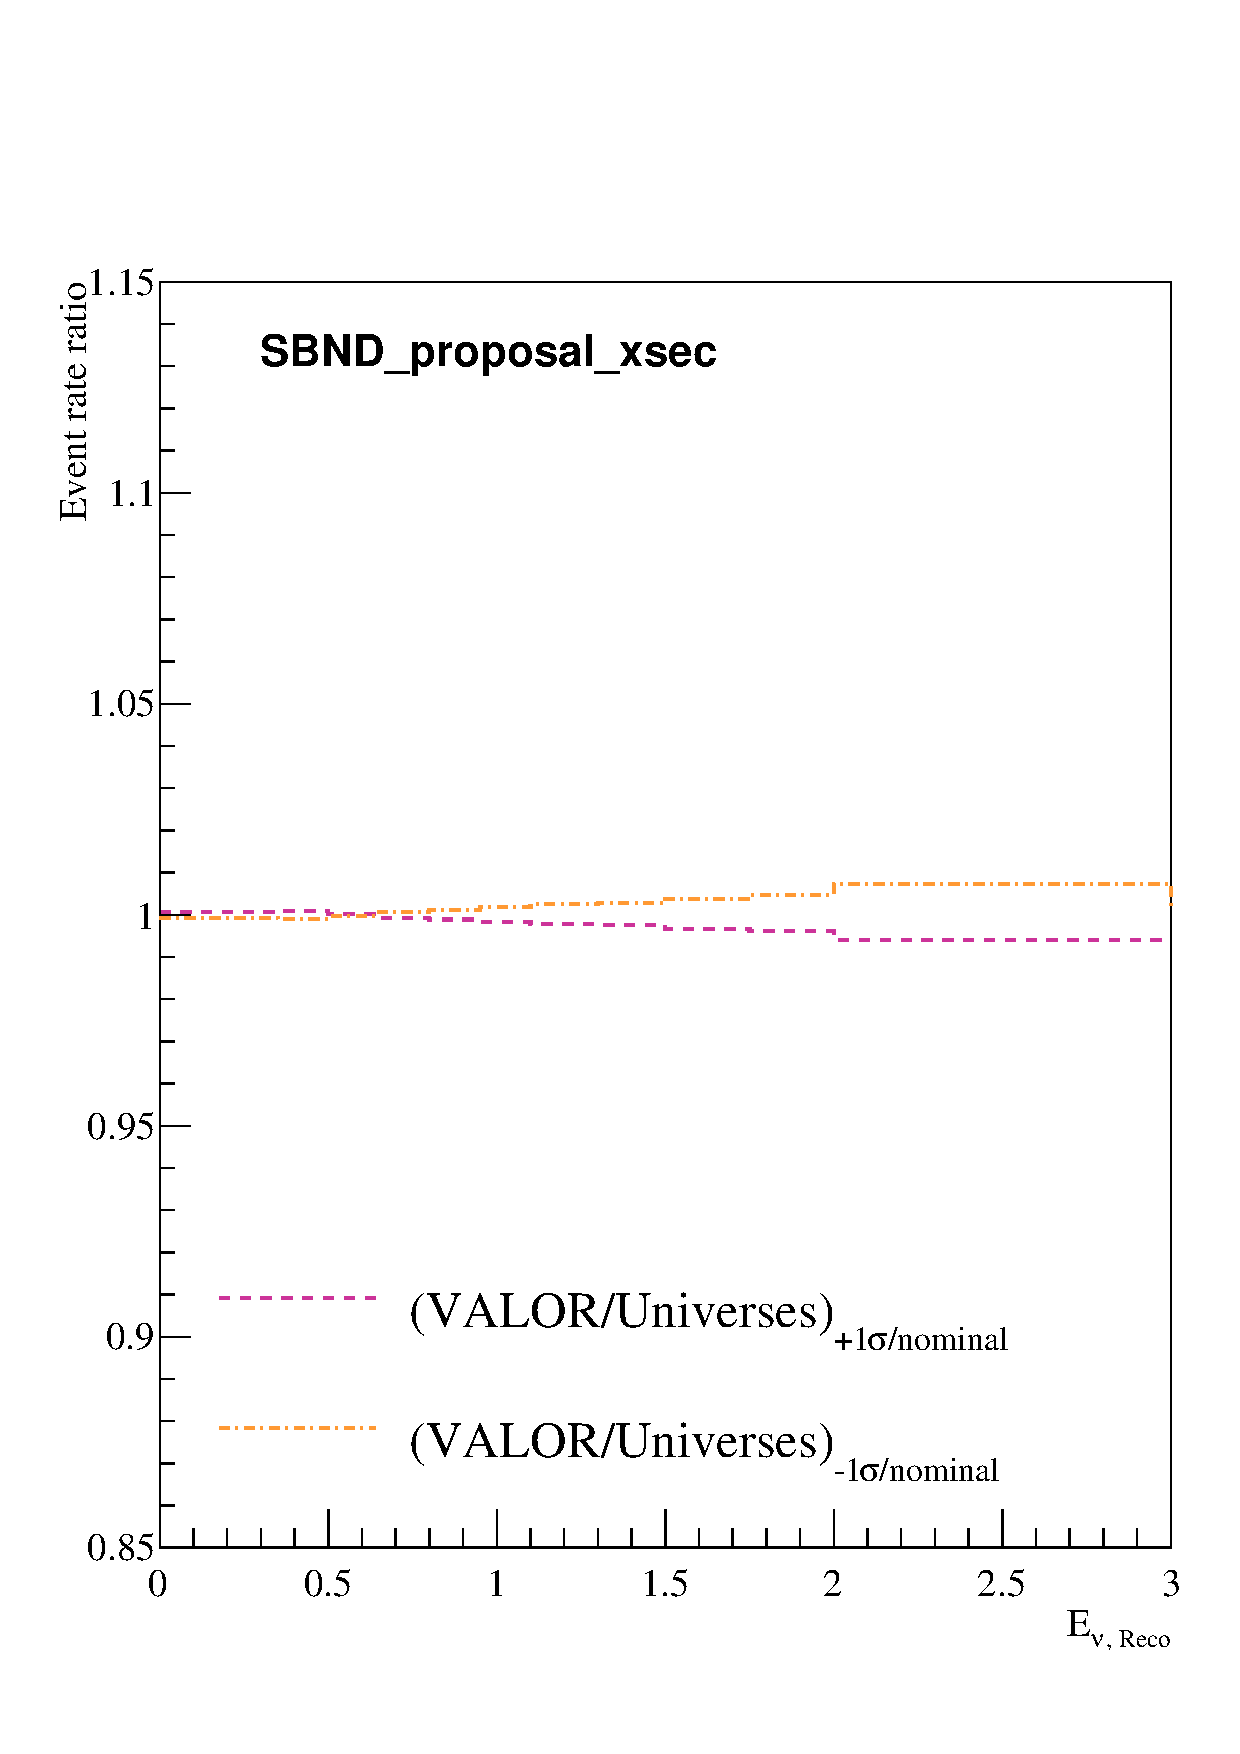
\includegraphics[width = \largefigwidth]{figures-chap5/tweak_pdf_N_nue/universe_valor_double_ratios_SBND_proposal_xsec.pdf}
    \caption{Caption}
    \label{fig:my_label}
\end{figure}

\begin{figure}
    \centering
    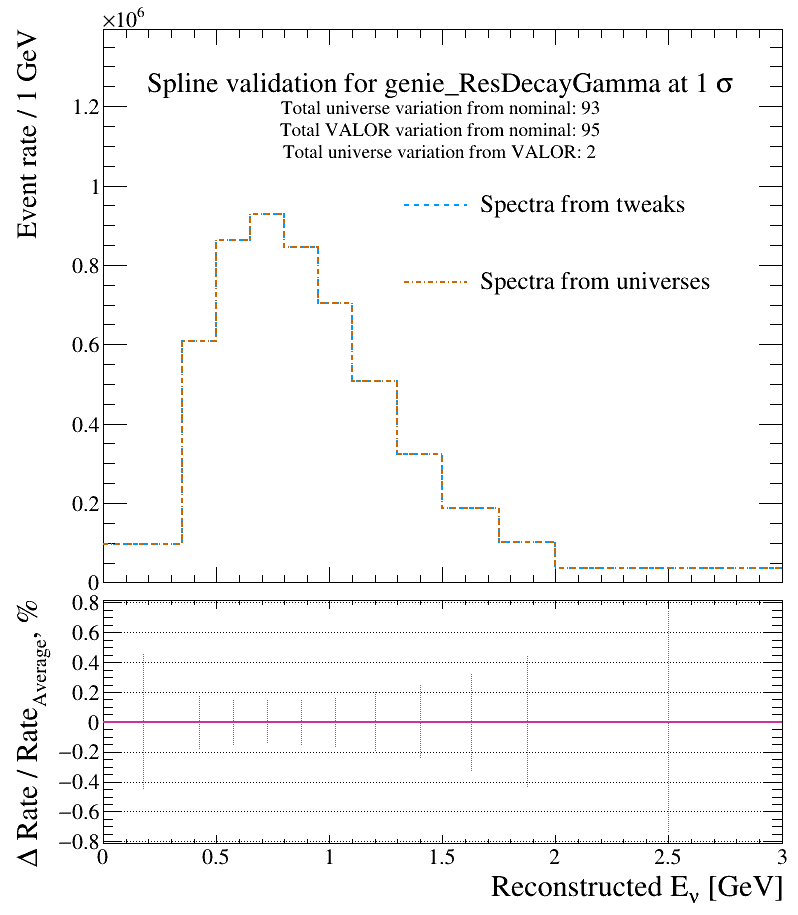
\includegraphics[width = \largefigwidth]{figures-chap5/tweak_nsigma_nue/genie_ResDecayGamma_Genie_nuelikeCChigh_1sigma_genie_ResDecayGamma_Genie.png}
    \caption[+1$\sigma$ variation comparison for the genie\_ResDecayGamma\_Genie parameter.]{A comparison of the +1$\sigma$ variation from the response functions in VALOR and the universes for the 'genie\_ResDecayGamma\_Genie' modern interaction systematic parameter.}
    \label{fig:my_label}
\end{figure}

\begin{figure}
    \centering
    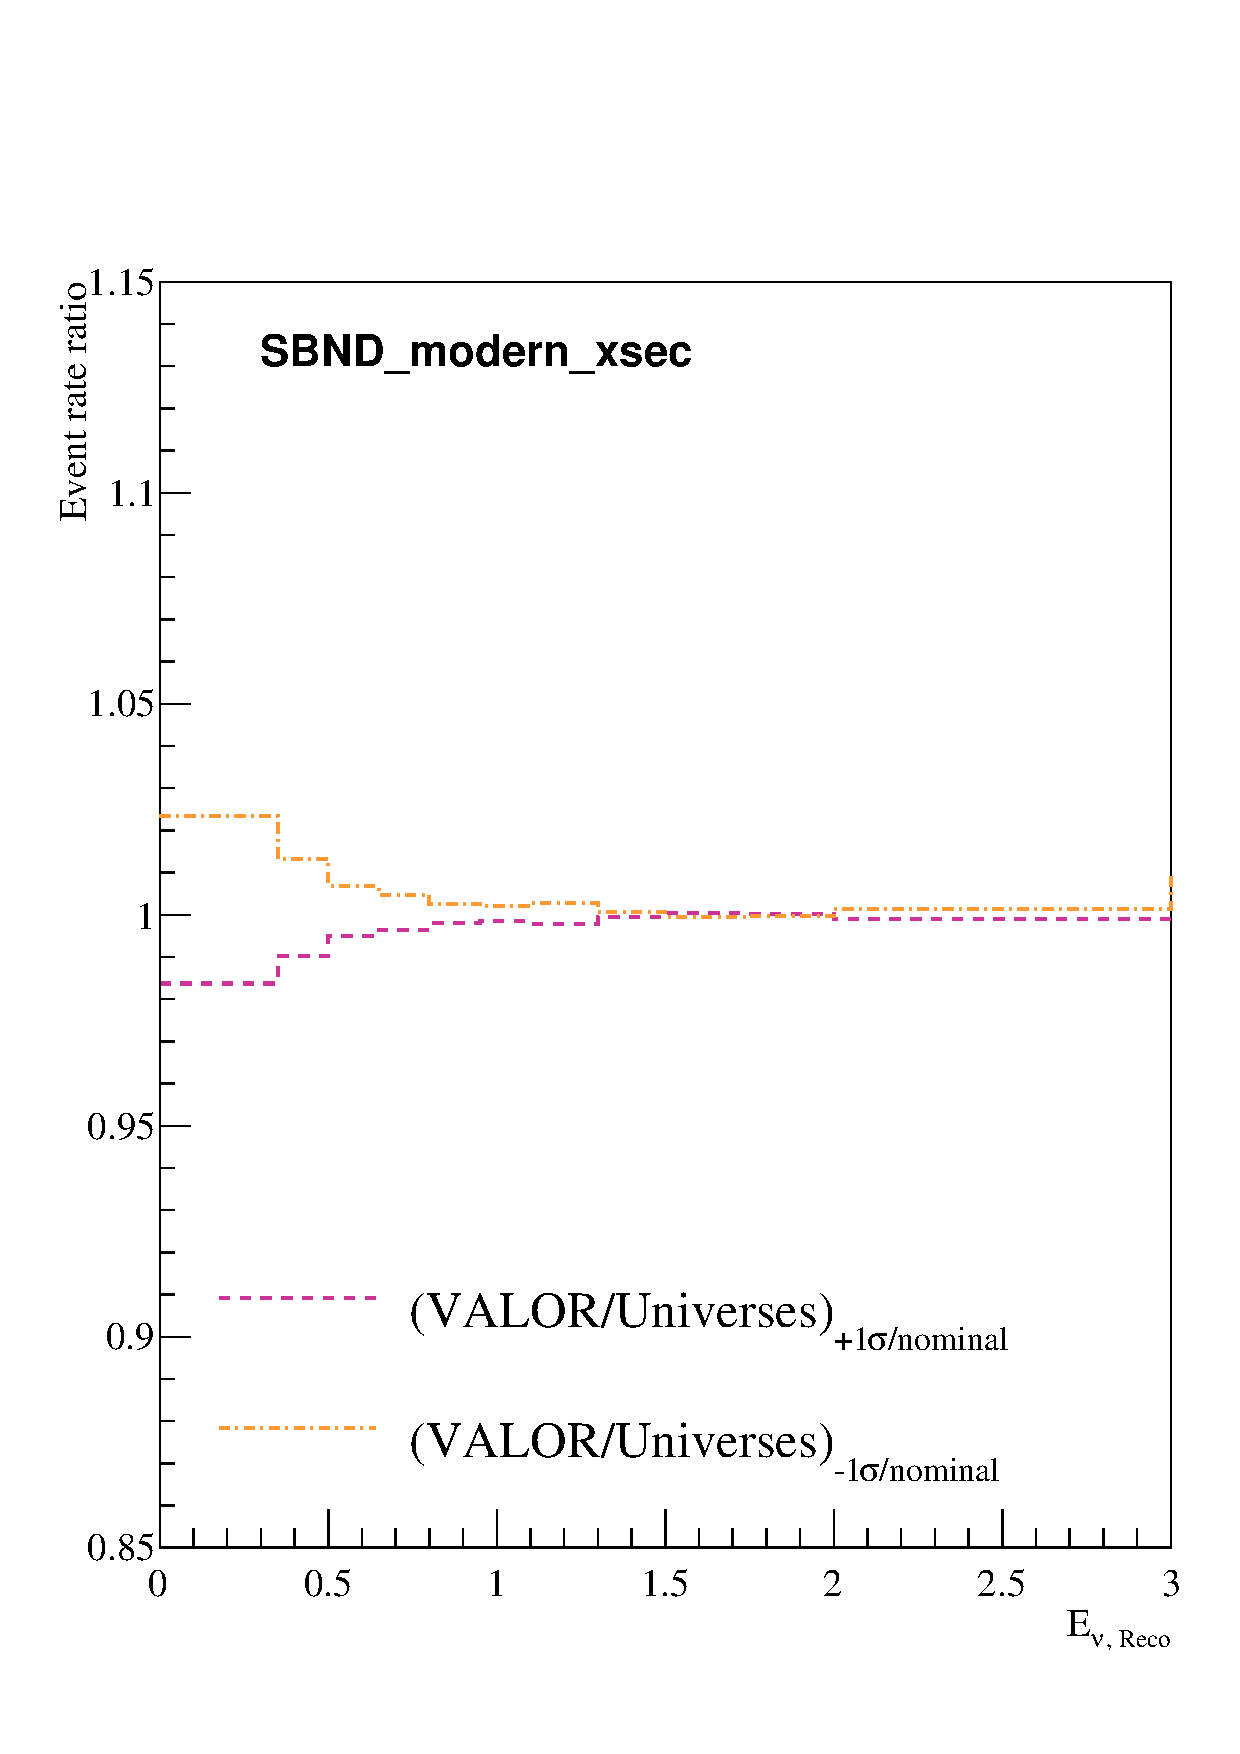
\includegraphics[width = \largefigwidth]{figures-chap5/tweak_pdf_N_nue/universe_valor_double_ratios_SBND_modern_xsec.pdf}
    \caption{Caption}
    \label{fig:my_label}
\end{figure}

\section{Other Systematics}
MEC, POT, Detector, Energy scale - maybe put some of these in above sections.
\section{Other Analysis Choices}
All the stuff that was 'agreed' between fitters - Baseline Approximation, Binning, Spectra energy range etc.

\subsection{Baseline}
As is shown in \EquationRef{eqn:sterile_osc_prob}, the baseline is one of the components that drives the oscillation probability. For long baseline experiments, it's not uncommon for fitting frameworks to simply use some average value for the baseline since factors such as the interaction point in the detector or the position at which a particle decays into a neutrino would only change the average baseline for the experiment by a negligible amount. However, for short baseline experiments such as \gls{sbn}, these factors may change the baseline significantly. 

In an attempt to minimise computing resources, the true baseline was not initially used, but instead several approximations to the baseline were tried. To begin with, the average baseline of each \gls{sbn} detector was used for all neutrino energies. This was calculated from the true baseline distribution of \numu events in each detector which are shown in \FigureRef{fig:numu_baseline}. Secondly, a 4-knot spline (named spline V1) for each detector was defined in order to try and better approximate the baseline. This method was improved upon by producing a spline for each of the true energy bins (named spline V2) which are defined in \SectionRef{sec:binning}. In order to establish the impact of any baseline approximations on the oscillation probability, the oscillation probability was plotted as a function of true neutrino energy with the oscillation parameters $sin^22\theta_{\mu\mu} = 0.01$ and $\Delta m^2_{41} = 50$ eV$^2$. This oscillation point was chosen to ensure that a region where rapid oscillation occur was being investigated, which would highlight the effect of any baseline choices. The oscillation probabilities as a function of energy are shown in \FigureRef{fig:baseline_osc_probability} for the four different baselines described. It was eventually decided that any approximation would be insufficient and that the true baseline should be used. 

The studies of the baseline approximations were done in the context of the \numu disappearance channel. For the \nue channels, different approximations should be applied, since the true baseline distribution is not the same as for \numu. In principal, within the \nue sample, different approximations should be applied to the different sub-samples since the baseline distribution is not the same for all the sub-samples. This was never done since it was decided that the true baseline should be used. Each individual sample used to construct the overall \nue event sample, has it's own baseline distribution due to the particles which contribute to each sample decaying at different points along the beamline. The baseline distribution for the intrinsic \nue, oscillated \nue and the overall \nue sample from combining all the sub-samples together is shown in \FigureRef{fig:nue_baseline_dist} for each of the \gls{sbn} detectors. It should be noted that the baseline distributions for oscillated \nue sample from \FigureRef{fig:nue_baseline_dist} and the \numu sample from \FigureRef{fig:numu_baseline} are comparable. This is due to the initial parameters describing the oscillated sample being the same as for the \numu sample. The only difference being the neutrino oscillations from \numu to \nue which isn't something that affects the baseline.

\begin{figure}[!h]
    \centering
    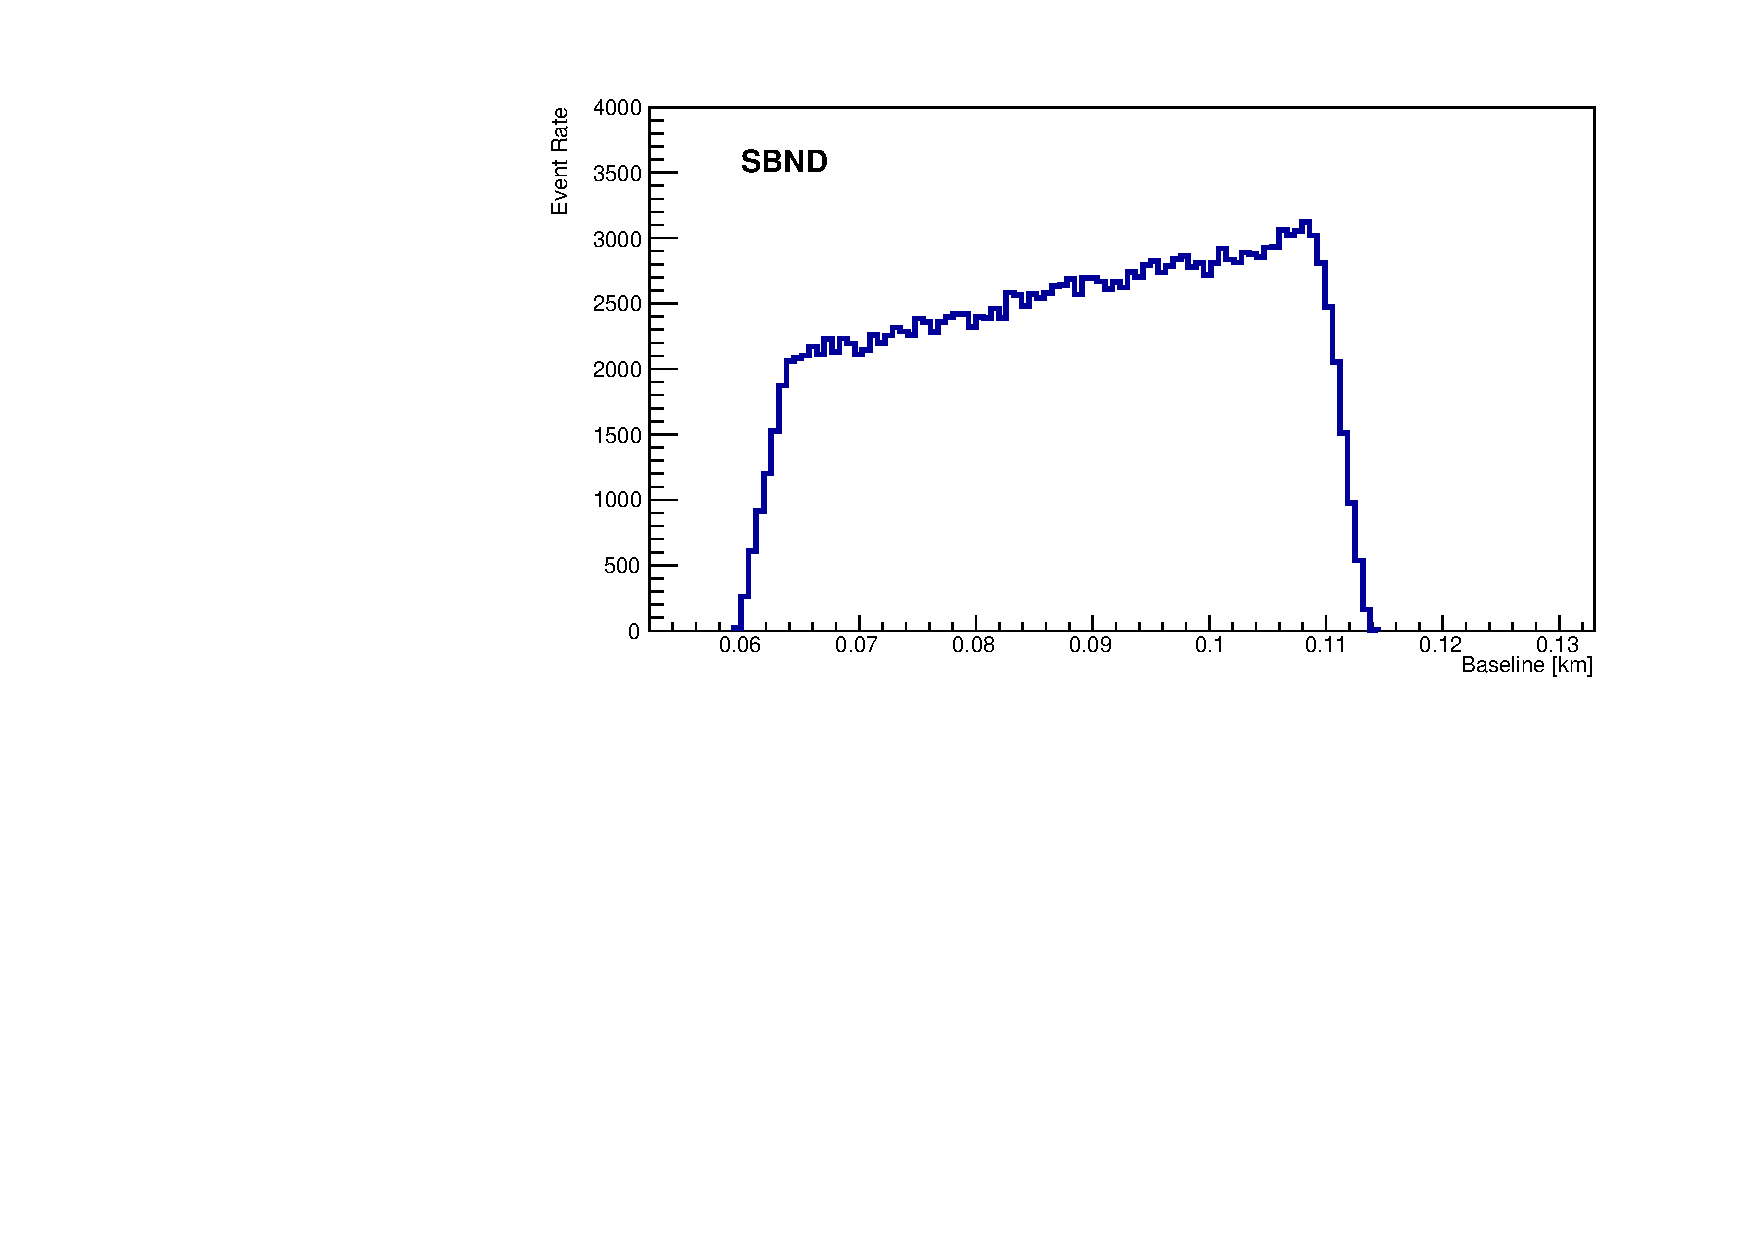
\includegraphics[width = 0.32\textwidth]{figures-chap5/SBND_numu.pdf}
    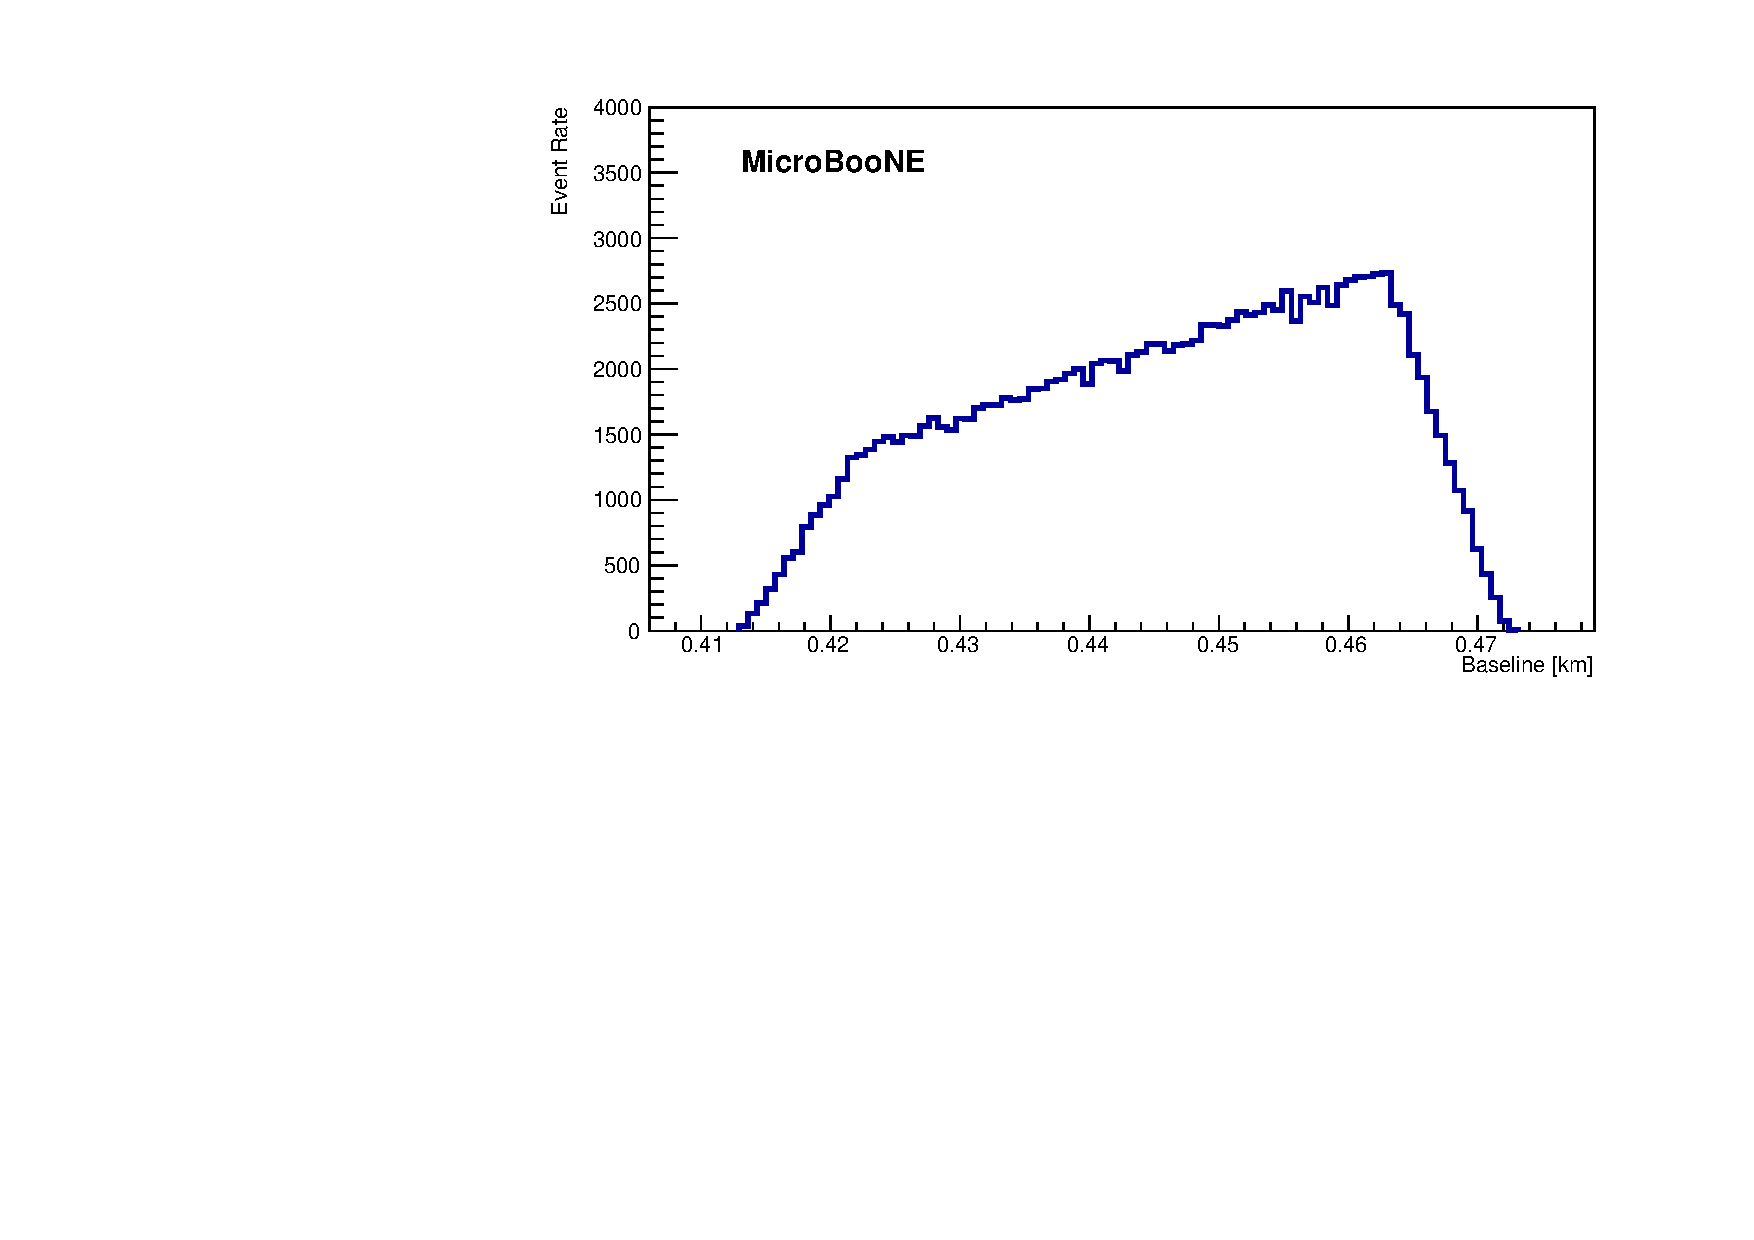
\includegraphics[width = 0.32\textwidth]{figures-chap5/MicroBooNE_numu.pdf}
    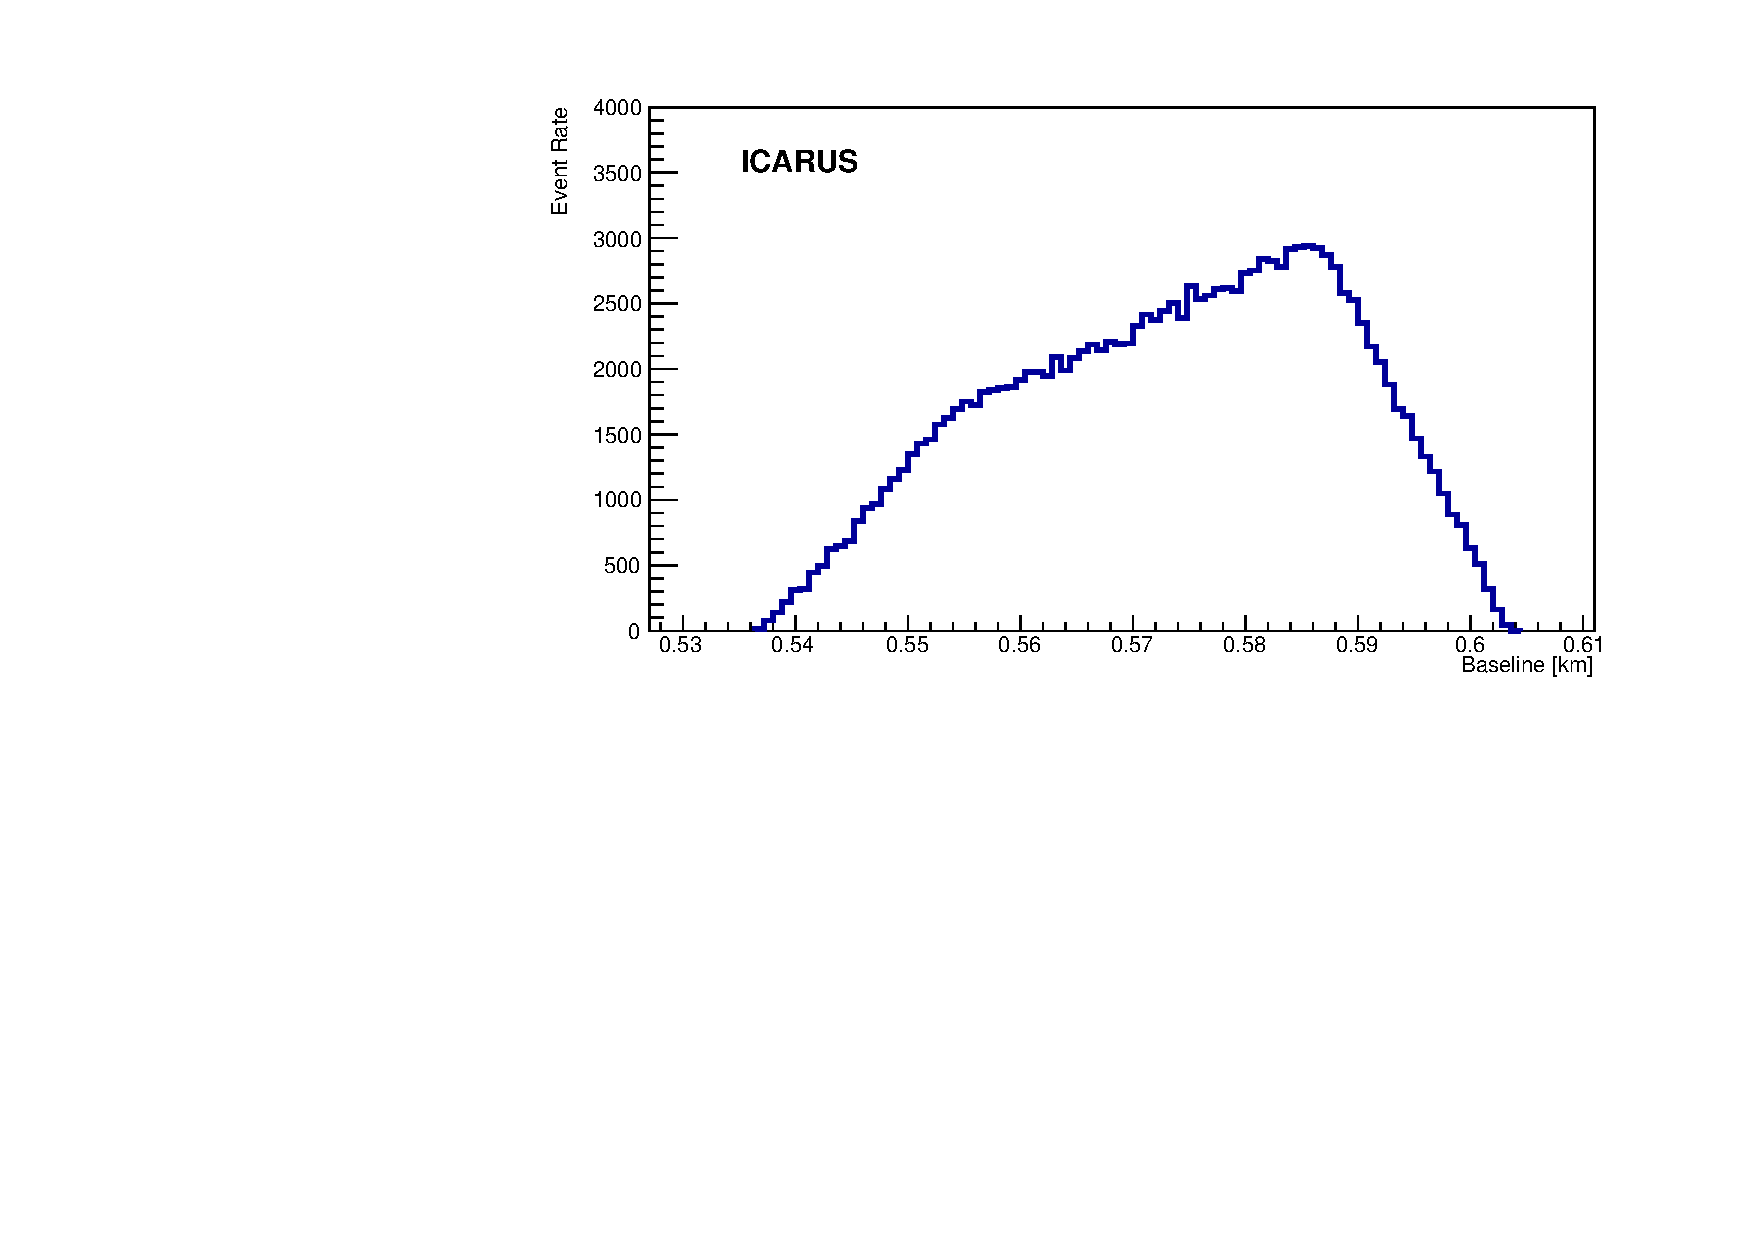
\includegraphics[width = 0.32\textwidth]{figures-chap5/ICARUS_numu.pdf}
    \caption{The baseline distribution of events in the \numu sample for each of the \gls{sbn} detectors.}
    \label{fig:numu_baseline}
\end{figure}

\begin{figure}[!h]
    \centering
    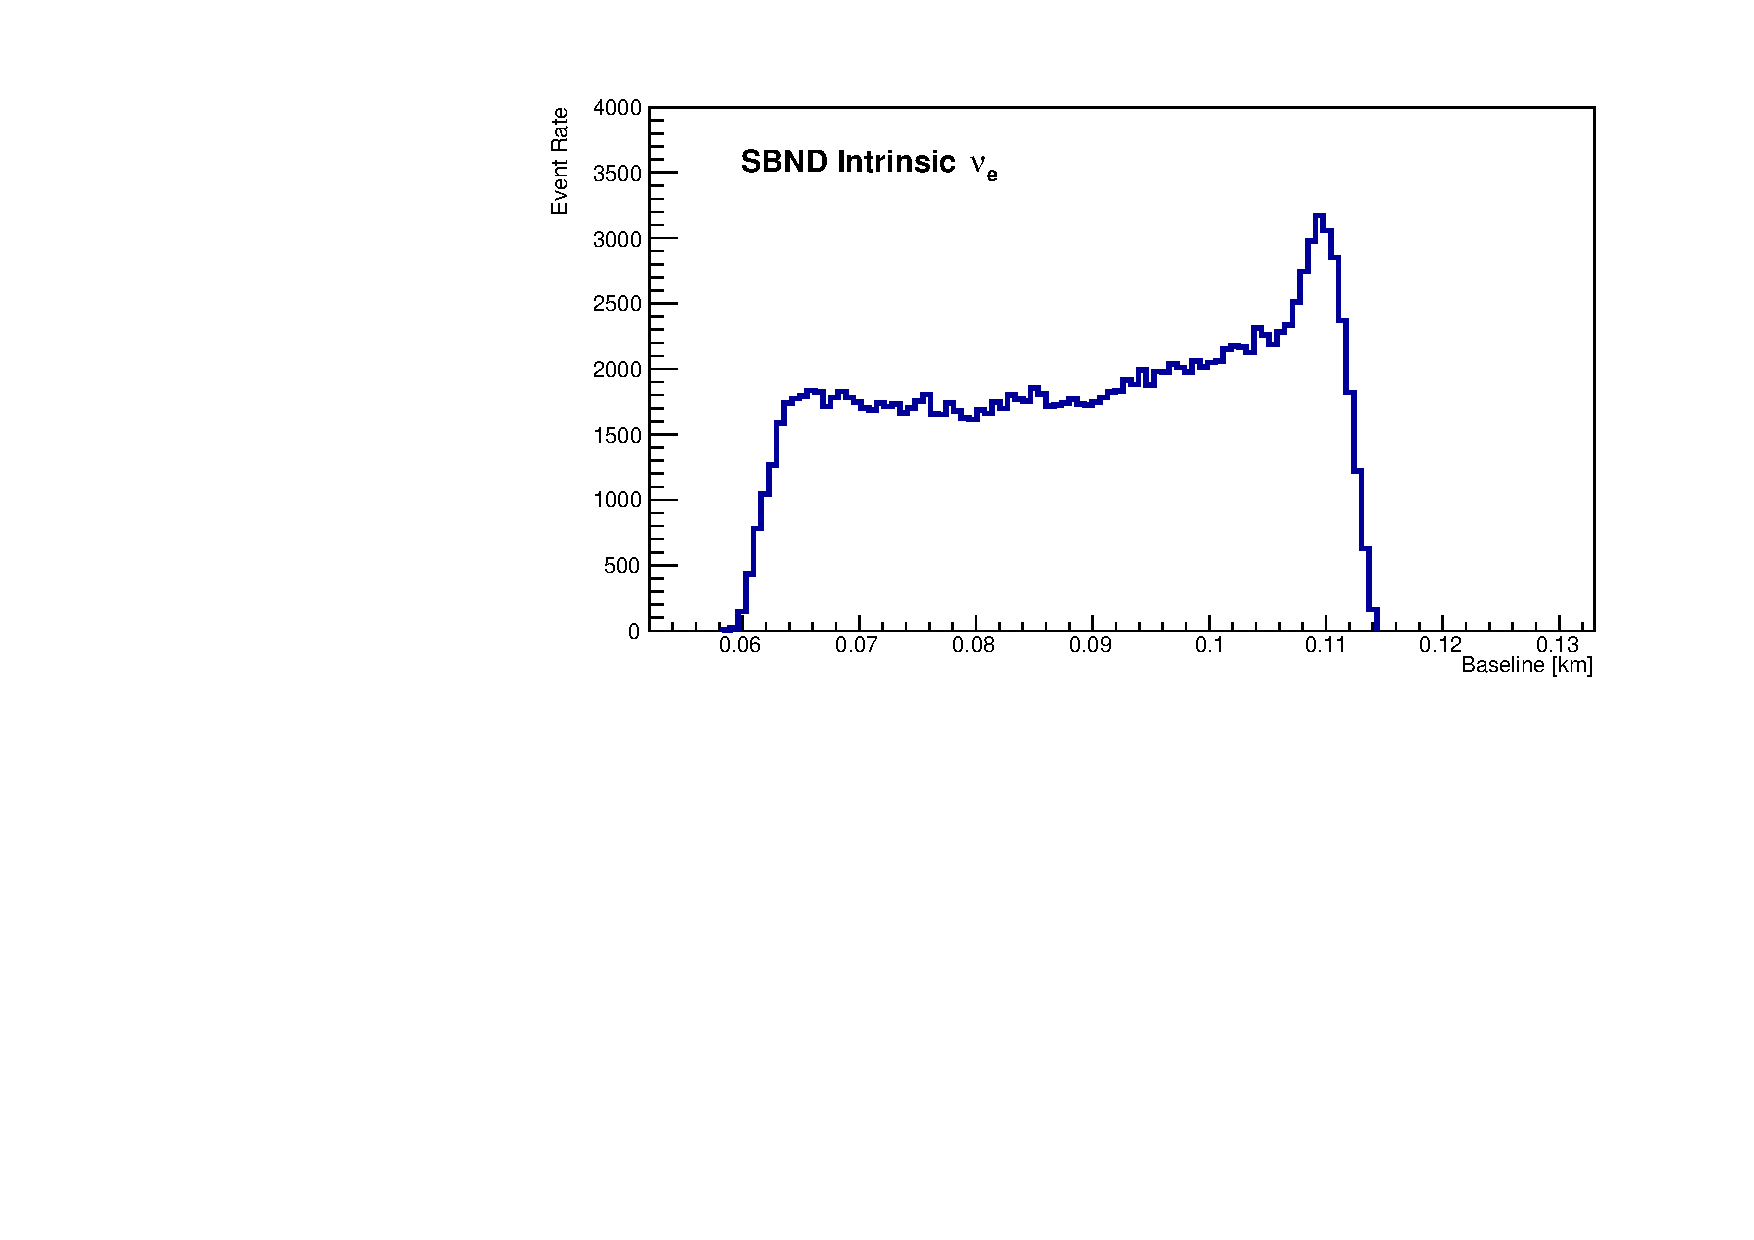
\includegraphics[width = 0.32\textwidth]{figures-chap5/SBND_intrinsic_nue.pdf}
    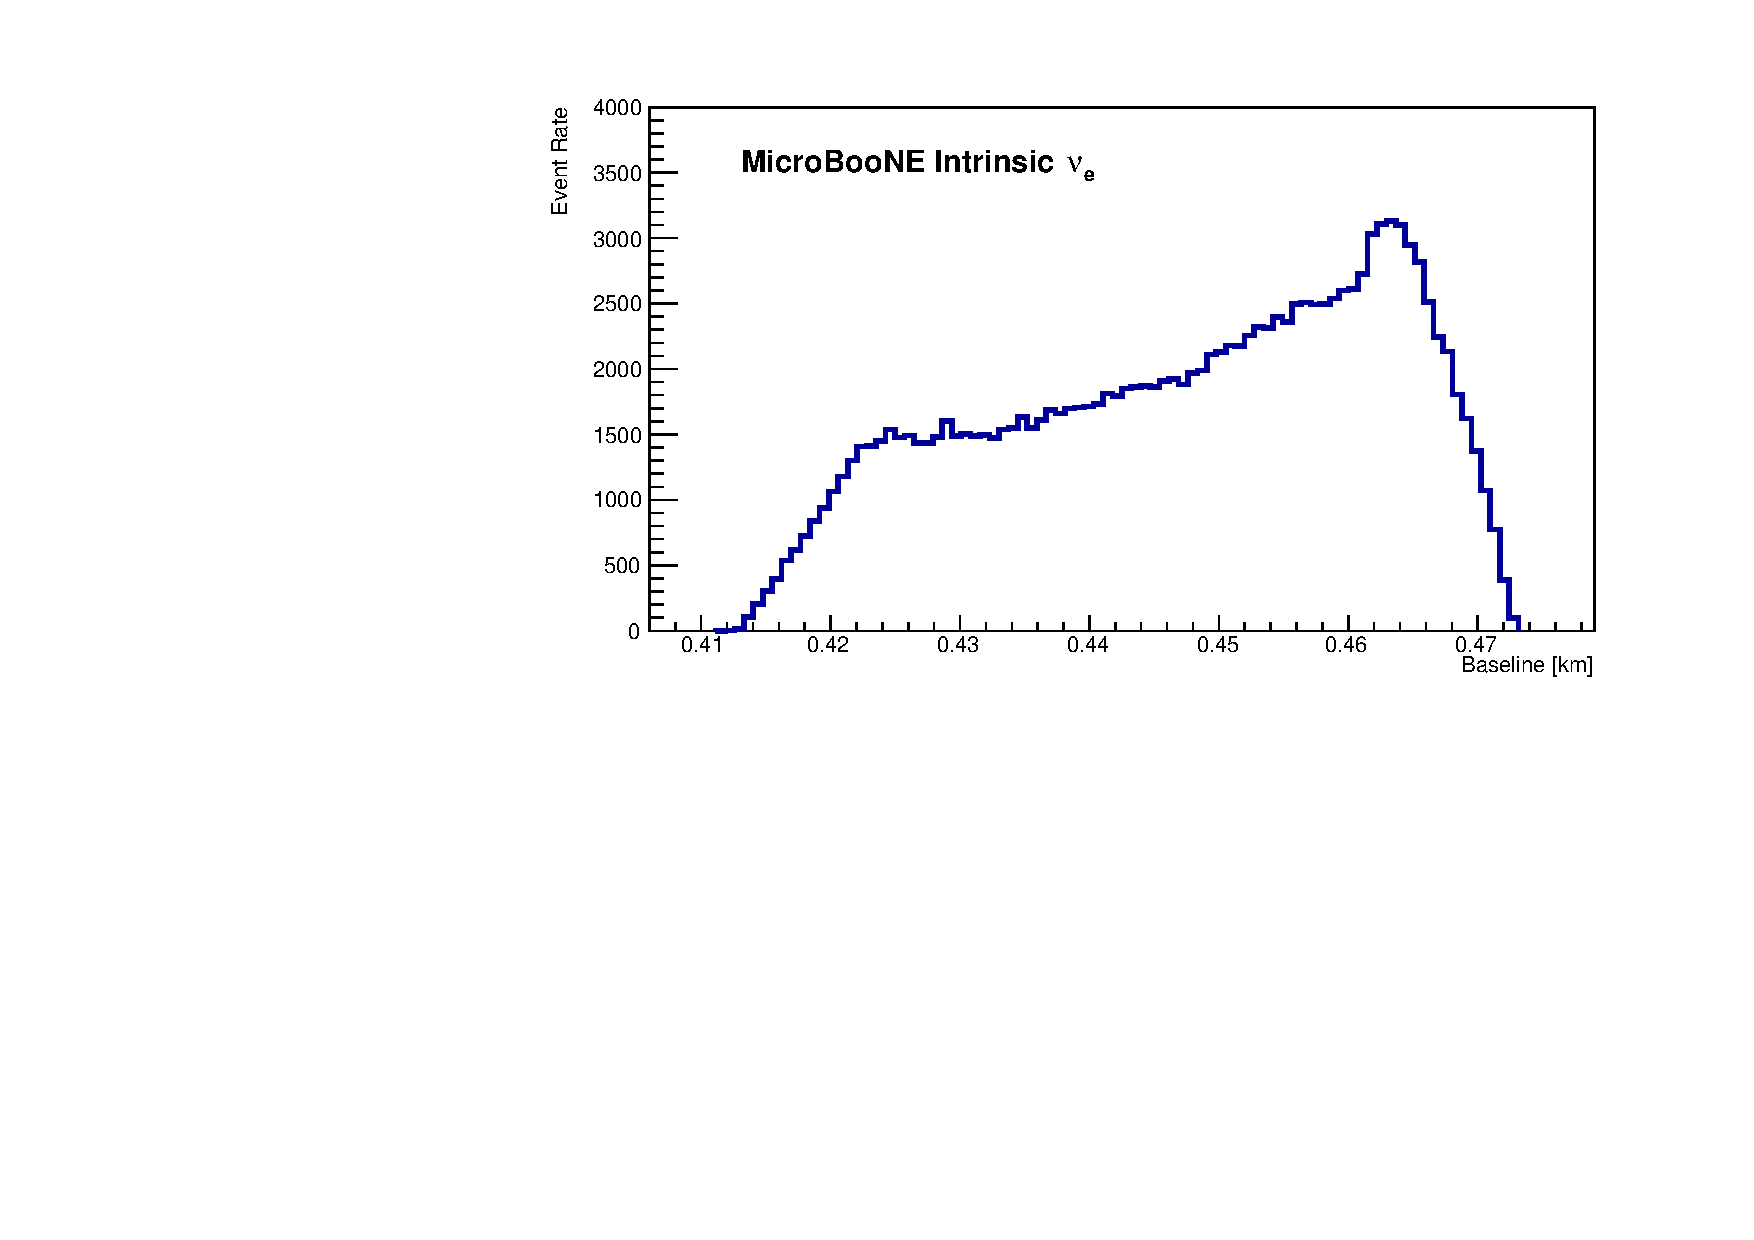
\includegraphics[width = 0.32\textwidth]{figures-chap5/MicroBooNE_intrinsic_nue.pdf}
    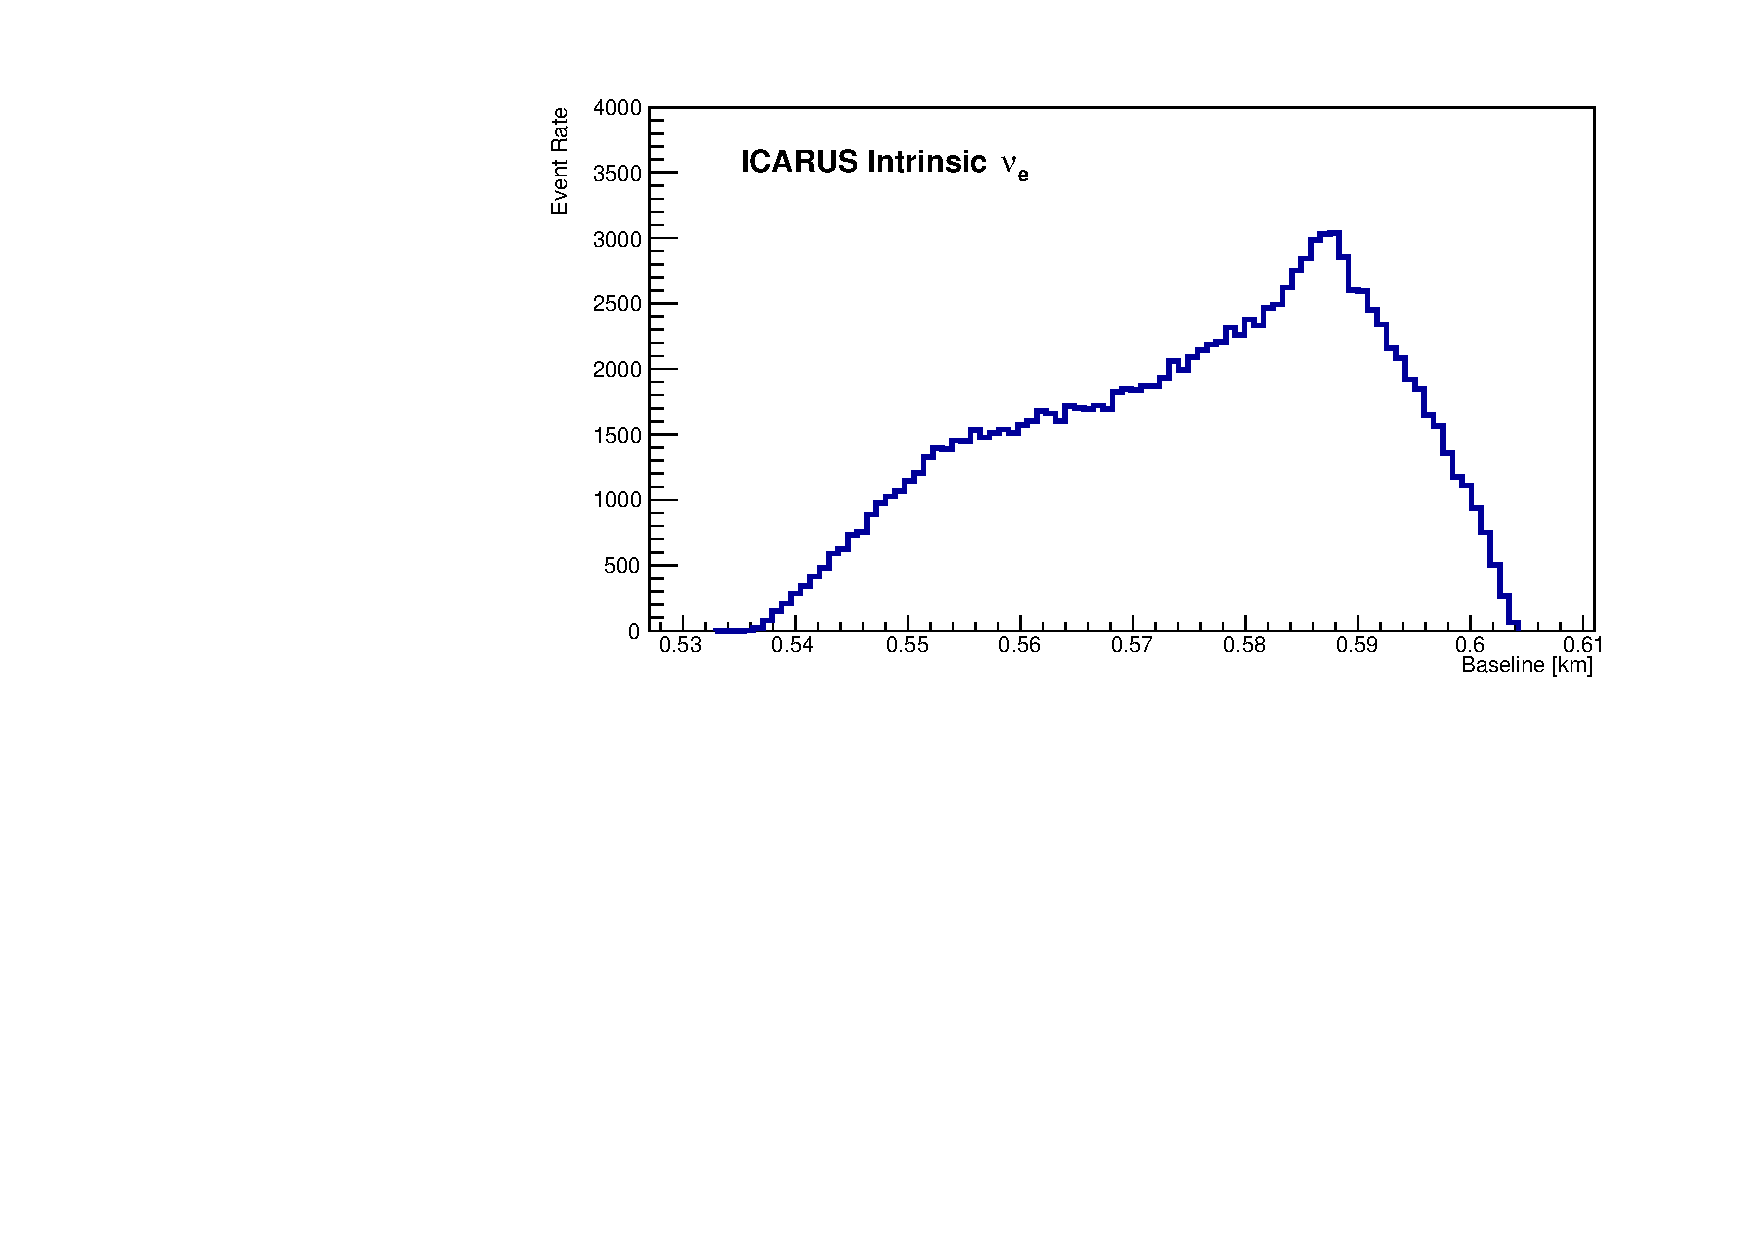
\includegraphics[width = 0.32\textwidth]{figures-chap5/ICARUS_intrinsic_nue.pdf} 
    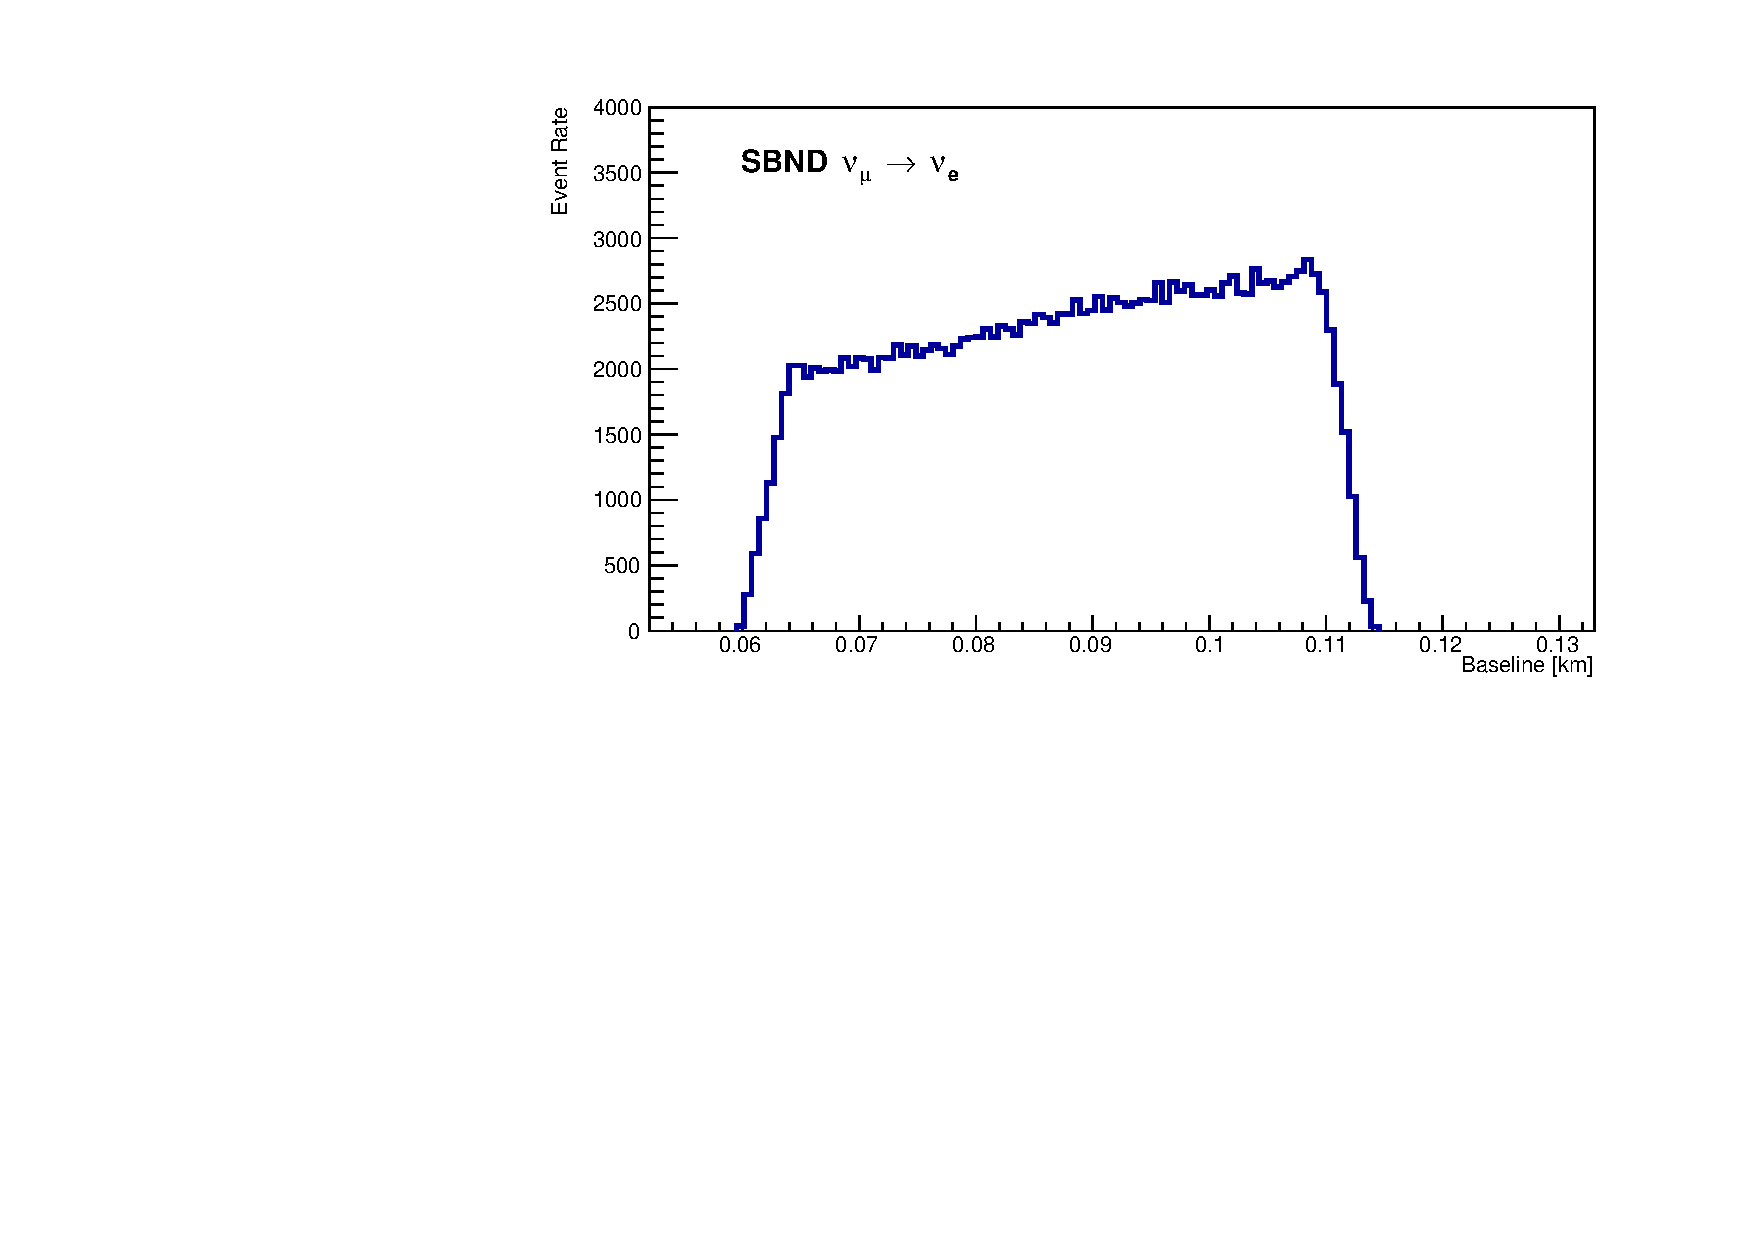
\includegraphics[width = 0.32\textwidth]{figures-chap5/SBND_osc.pdf}
    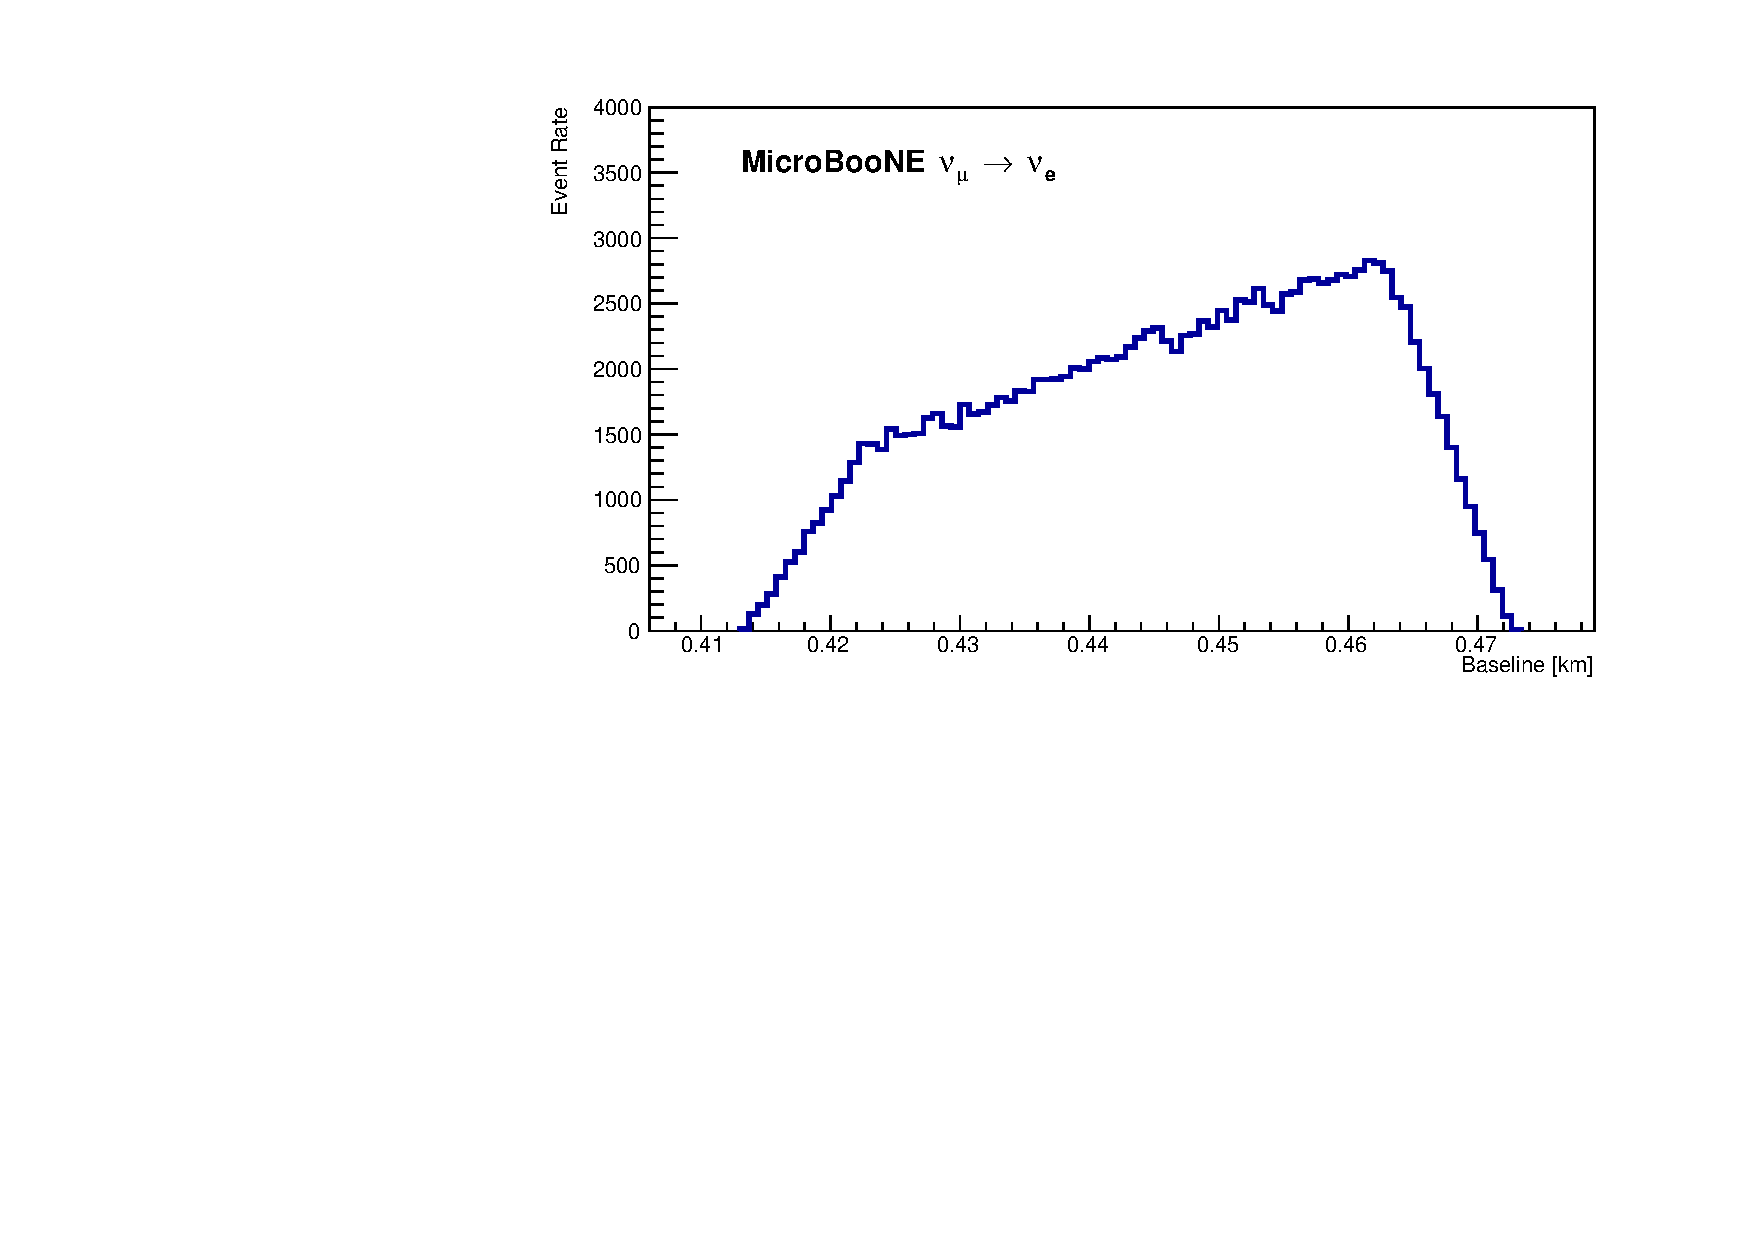
\includegraphics[width = 0.32\textwidth]{figures-chap5/MicroBooNE_osc.pdf}
    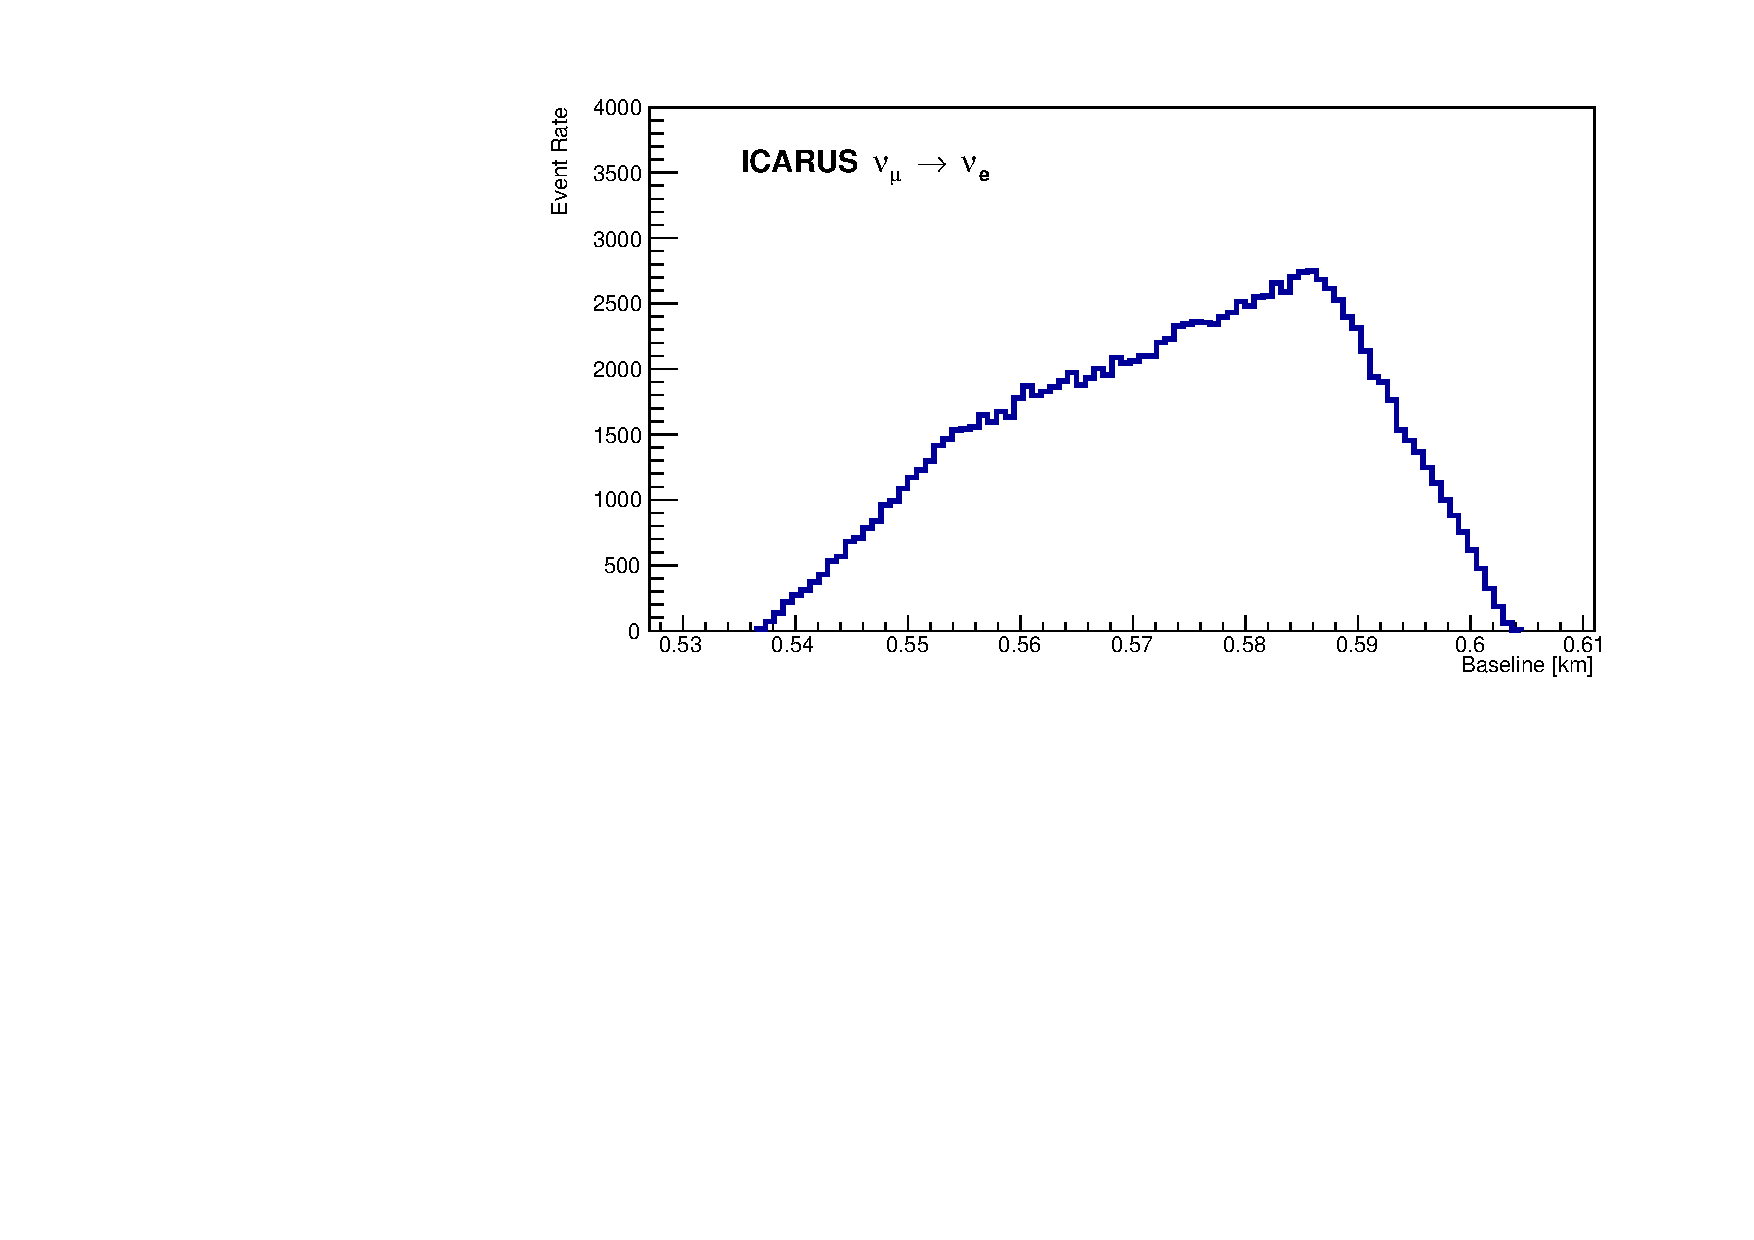
\includegraphics[width = 0.32\textwidth]{figures-chap5/ICARUS_osc.pdf}
    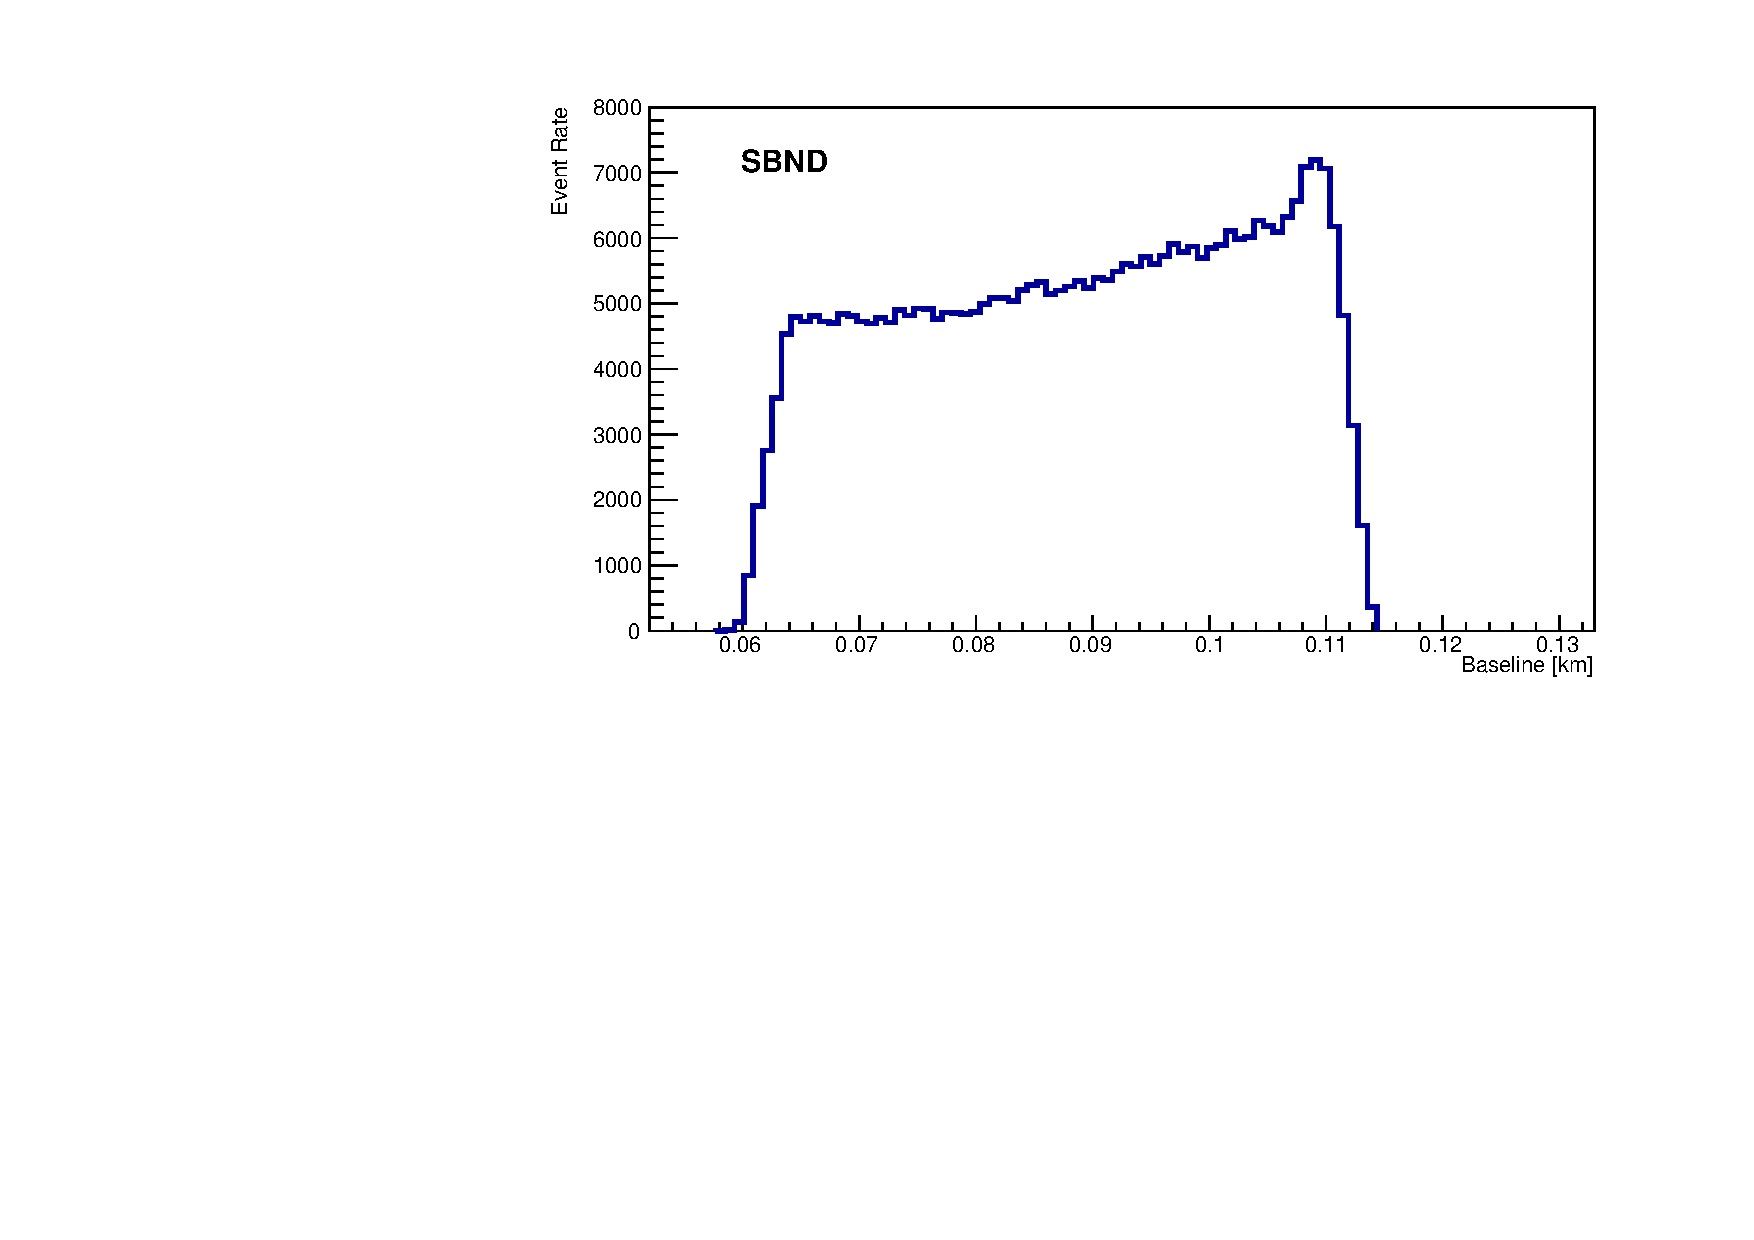
\includegraphics[width = 0.32\textwidth]{figures-chap5/SBND_nue.pdf}
    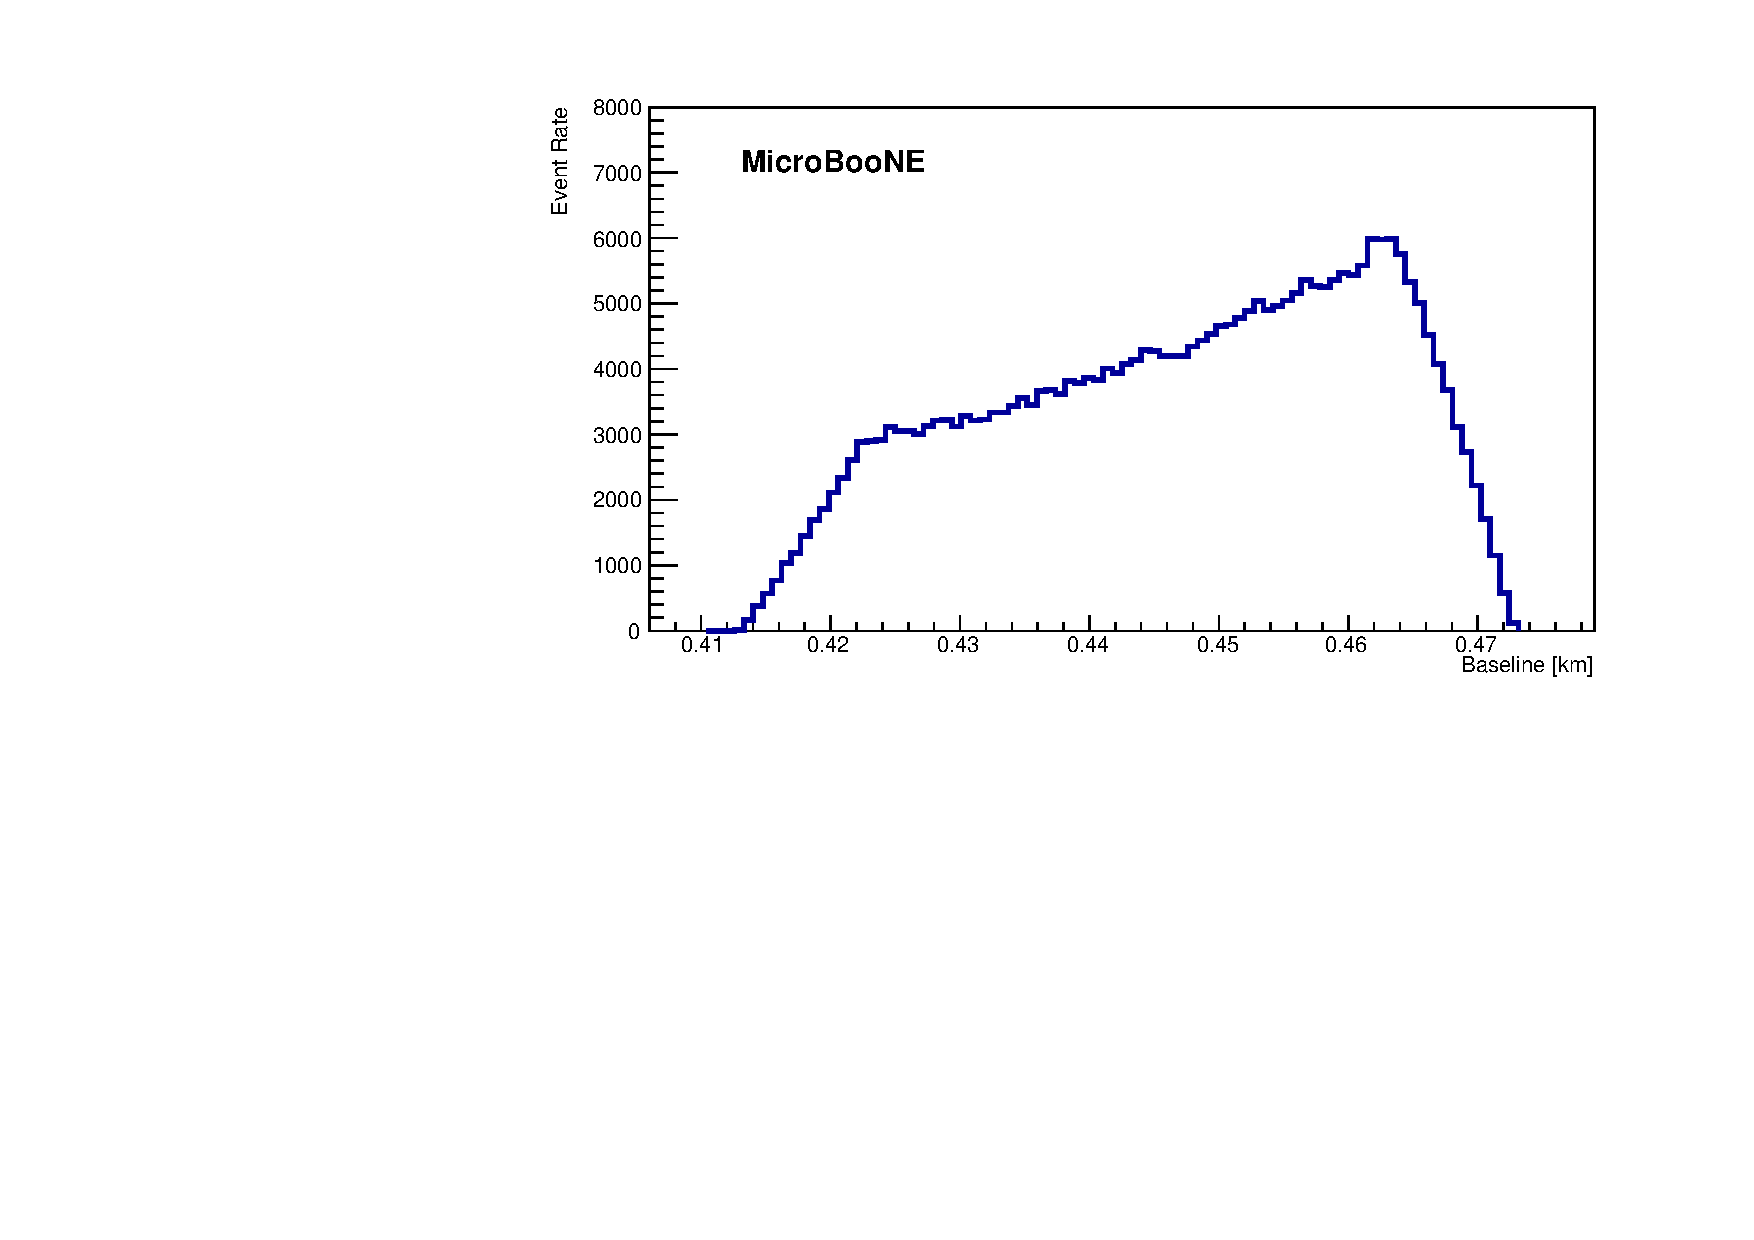
\includegraphics[width = 0.32\textwidth]{figures-chap5/MicroBooNE_nue.pdf}
    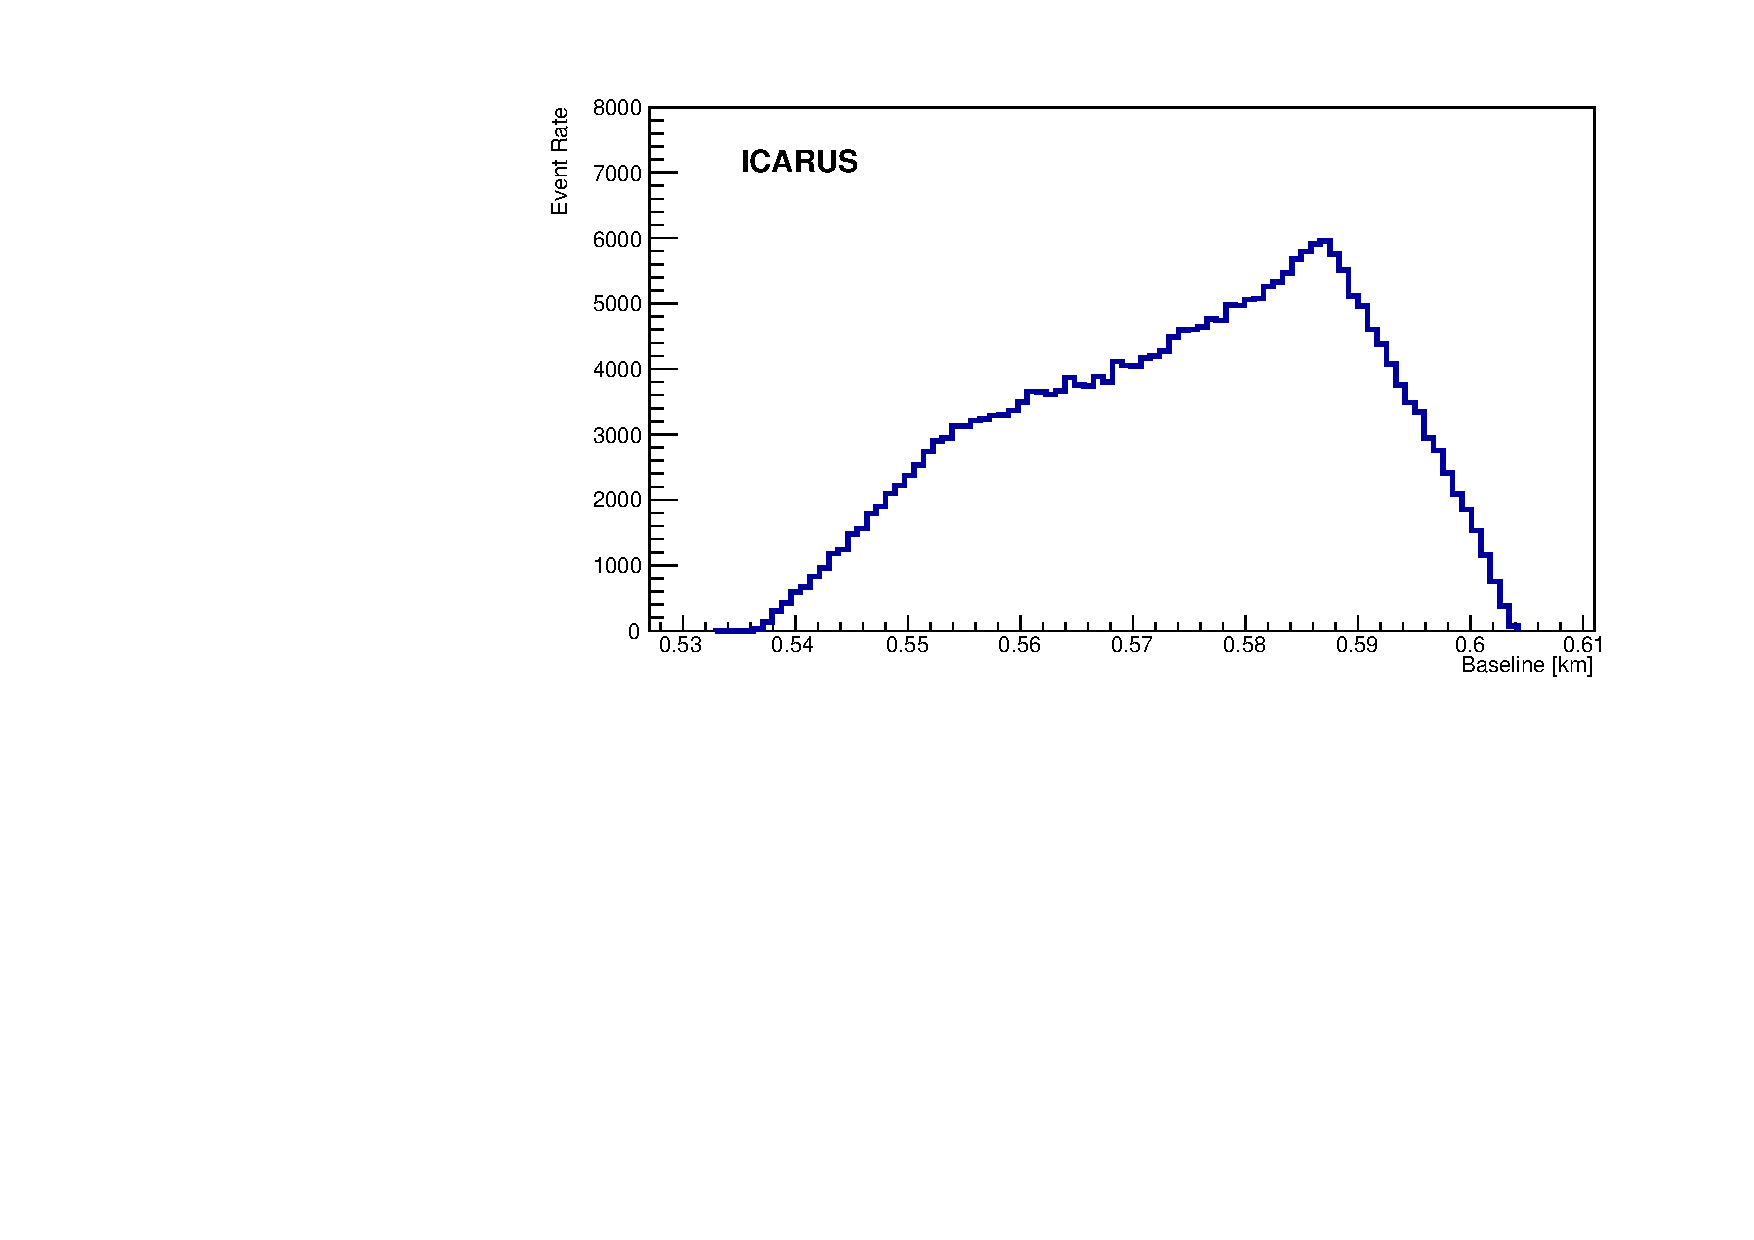
\includegraphics[width = 0.32\textwidth]{figures-chap5/ICARUS_nue.pdf}
    \caption{The baseline distribution of events in each of the \gls{sbn} detectors for the intrinsic \nue sample (Top), the oscillated \nue sample (Middle) and the overall \nue sample (Bottom). The overall sample is comprised of the events from the intrinsic \nue, oscillated \nue, the \numu events from \FigureRef{fig:numu_baseline} passing the \nue selection and the dirt and cosmic samples (which are not explicitly shown).
    The overall baseline distribution for events used in the \nue sample in each of the three \gls{sbn} detectors.}
    \label{fig:nue_baseline_dist}
\end{figure}

\begin{figure}[!h]
    \centering
    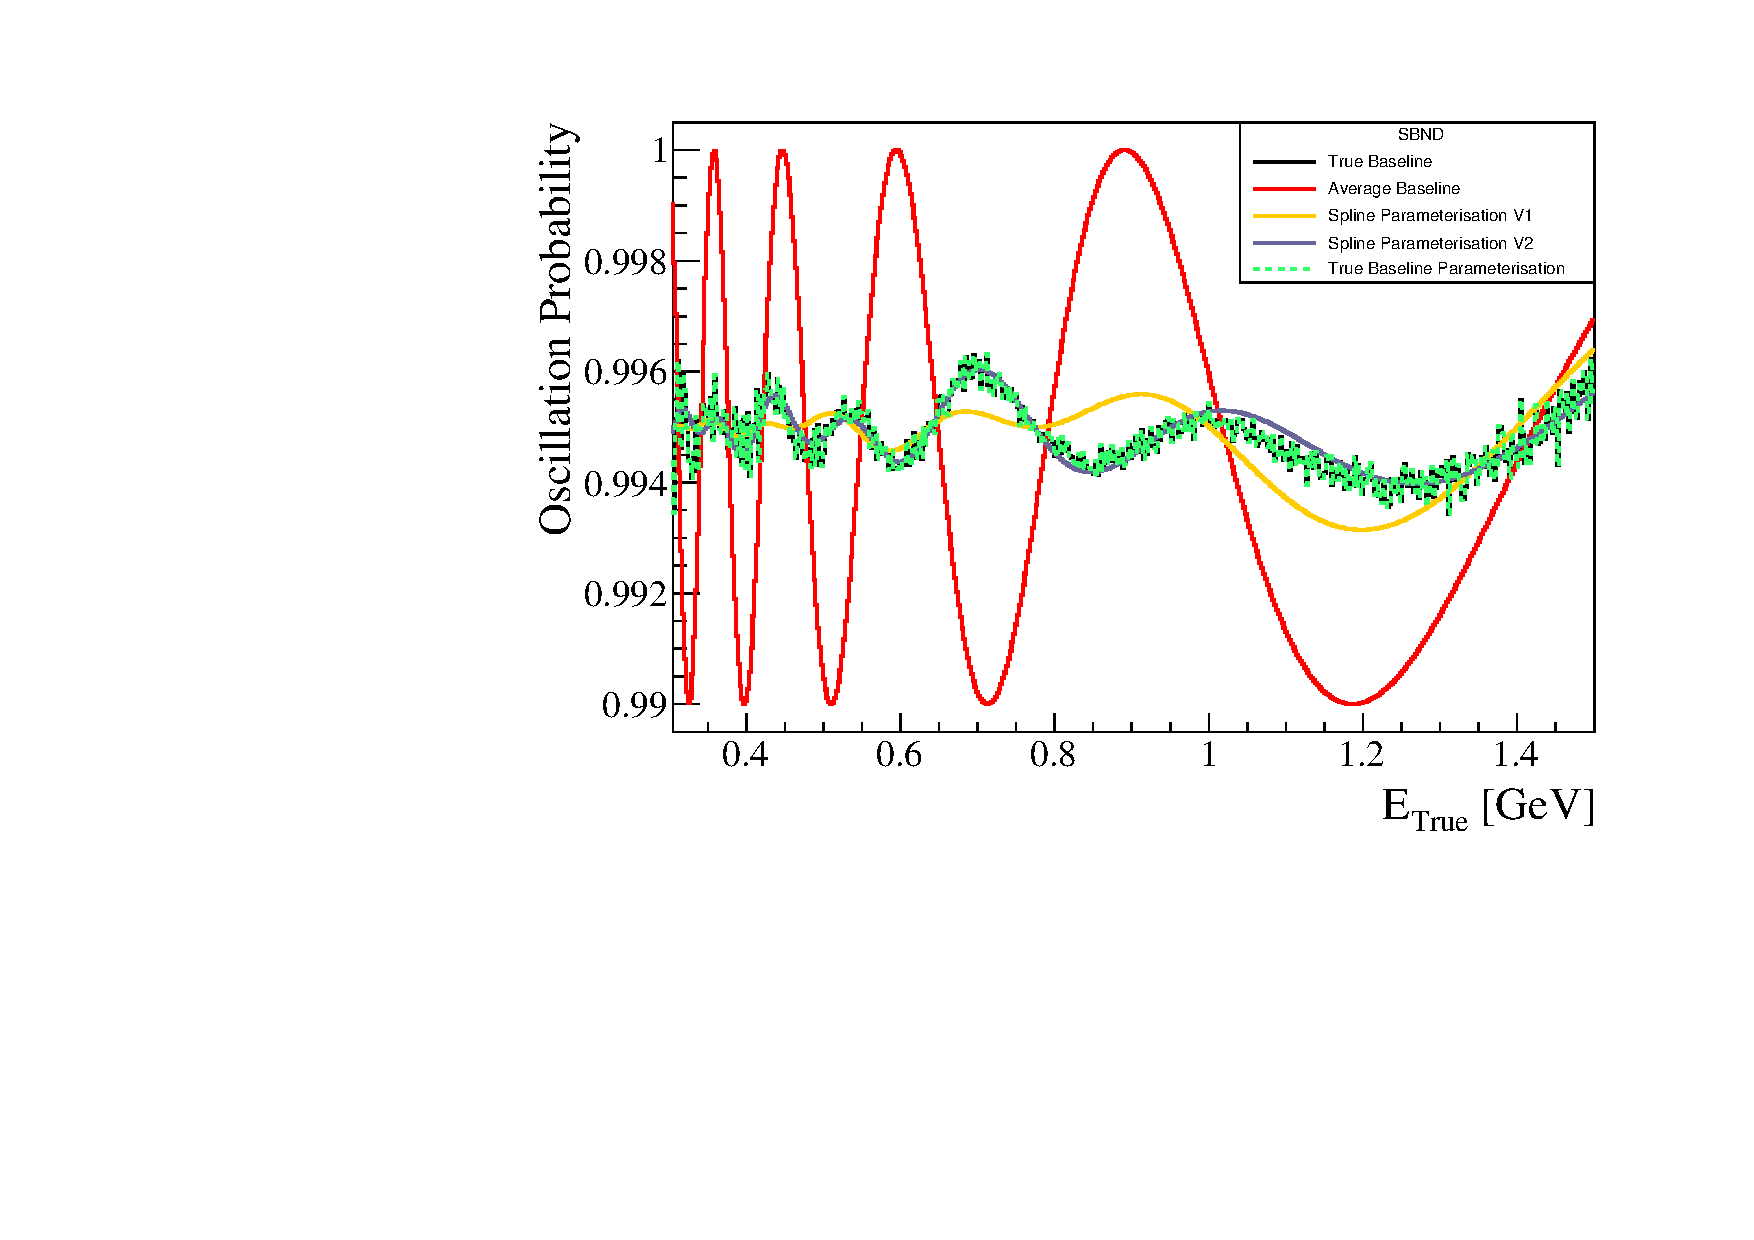
\includegraphics[width = 0.32\textwidth]{figures-chap5/osc_prob_sbnd.pdf}
    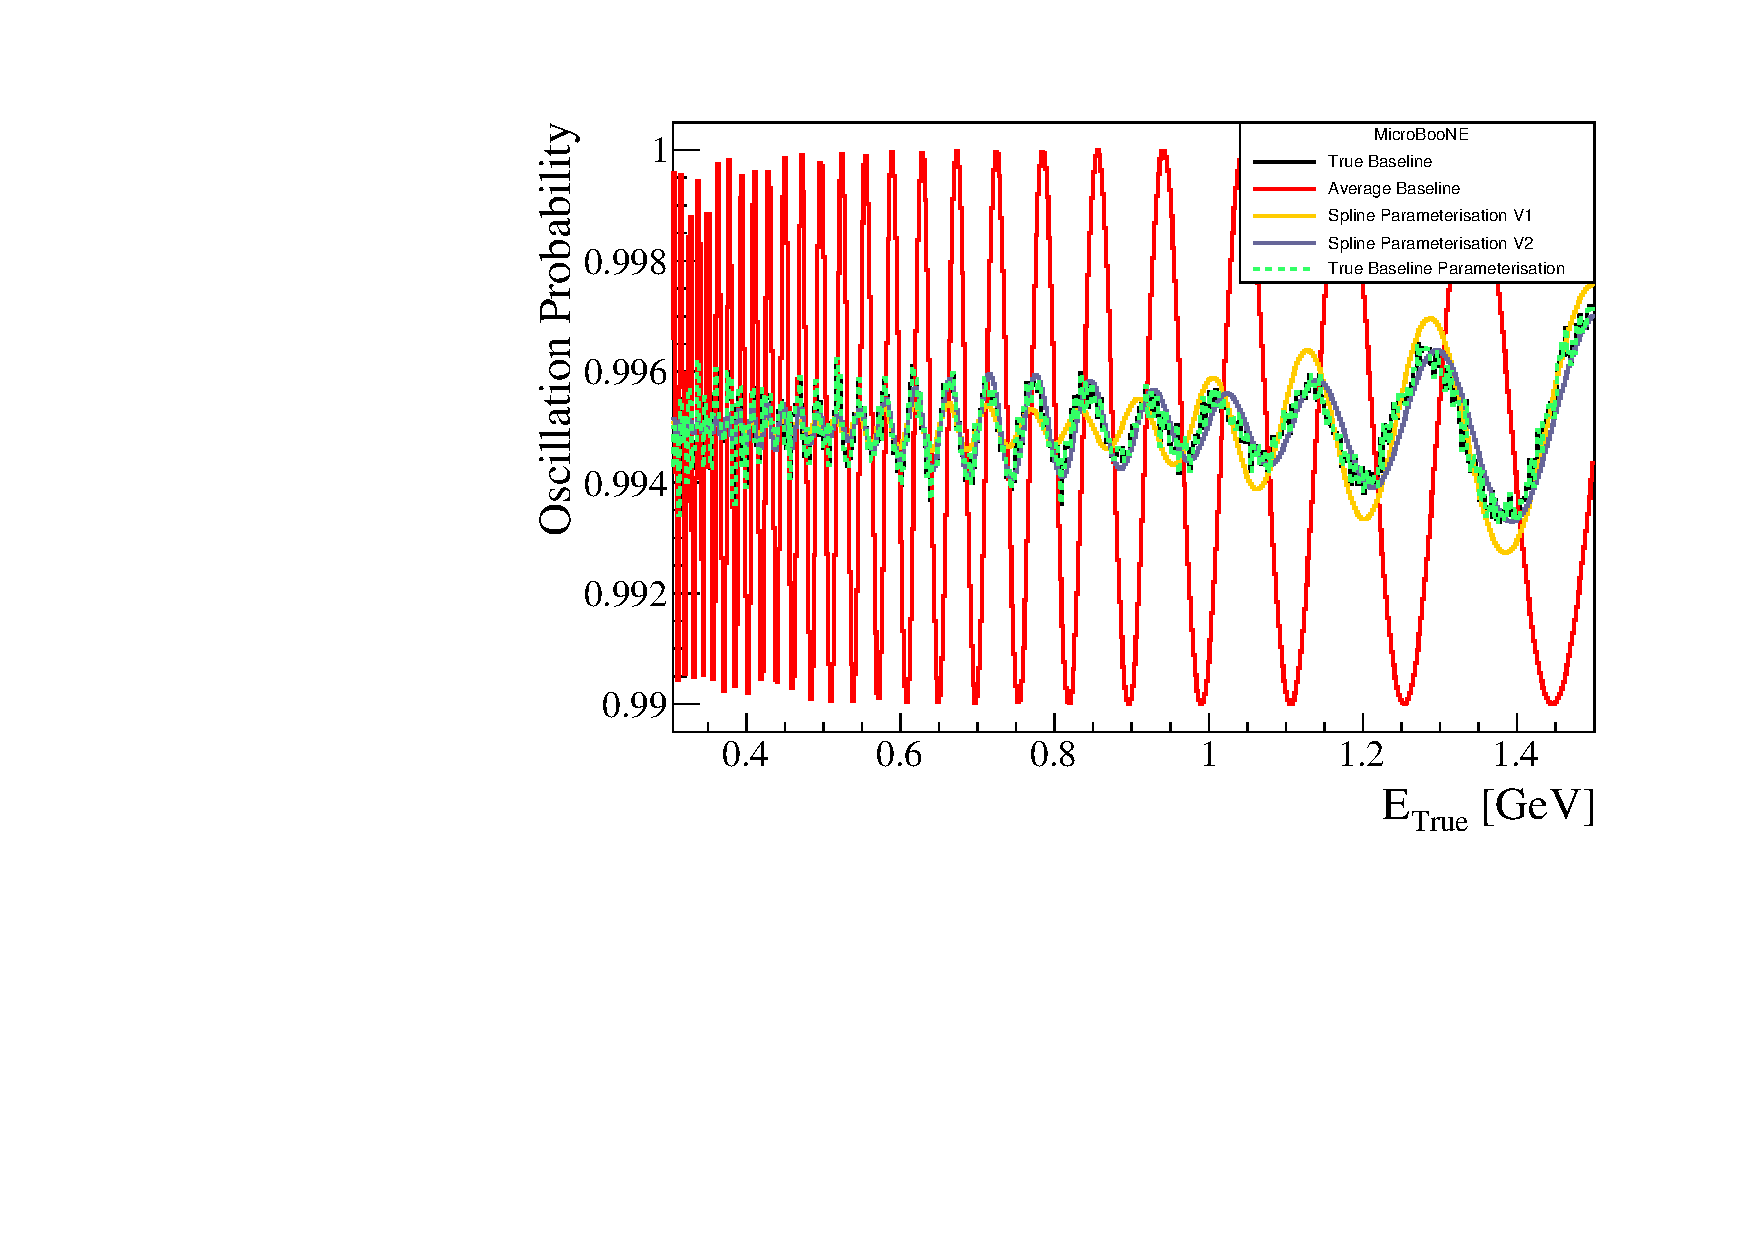
\includegraphics[width = 0.32\textwidth]{figures-chap5/osc_prob_uboone.pdf}
    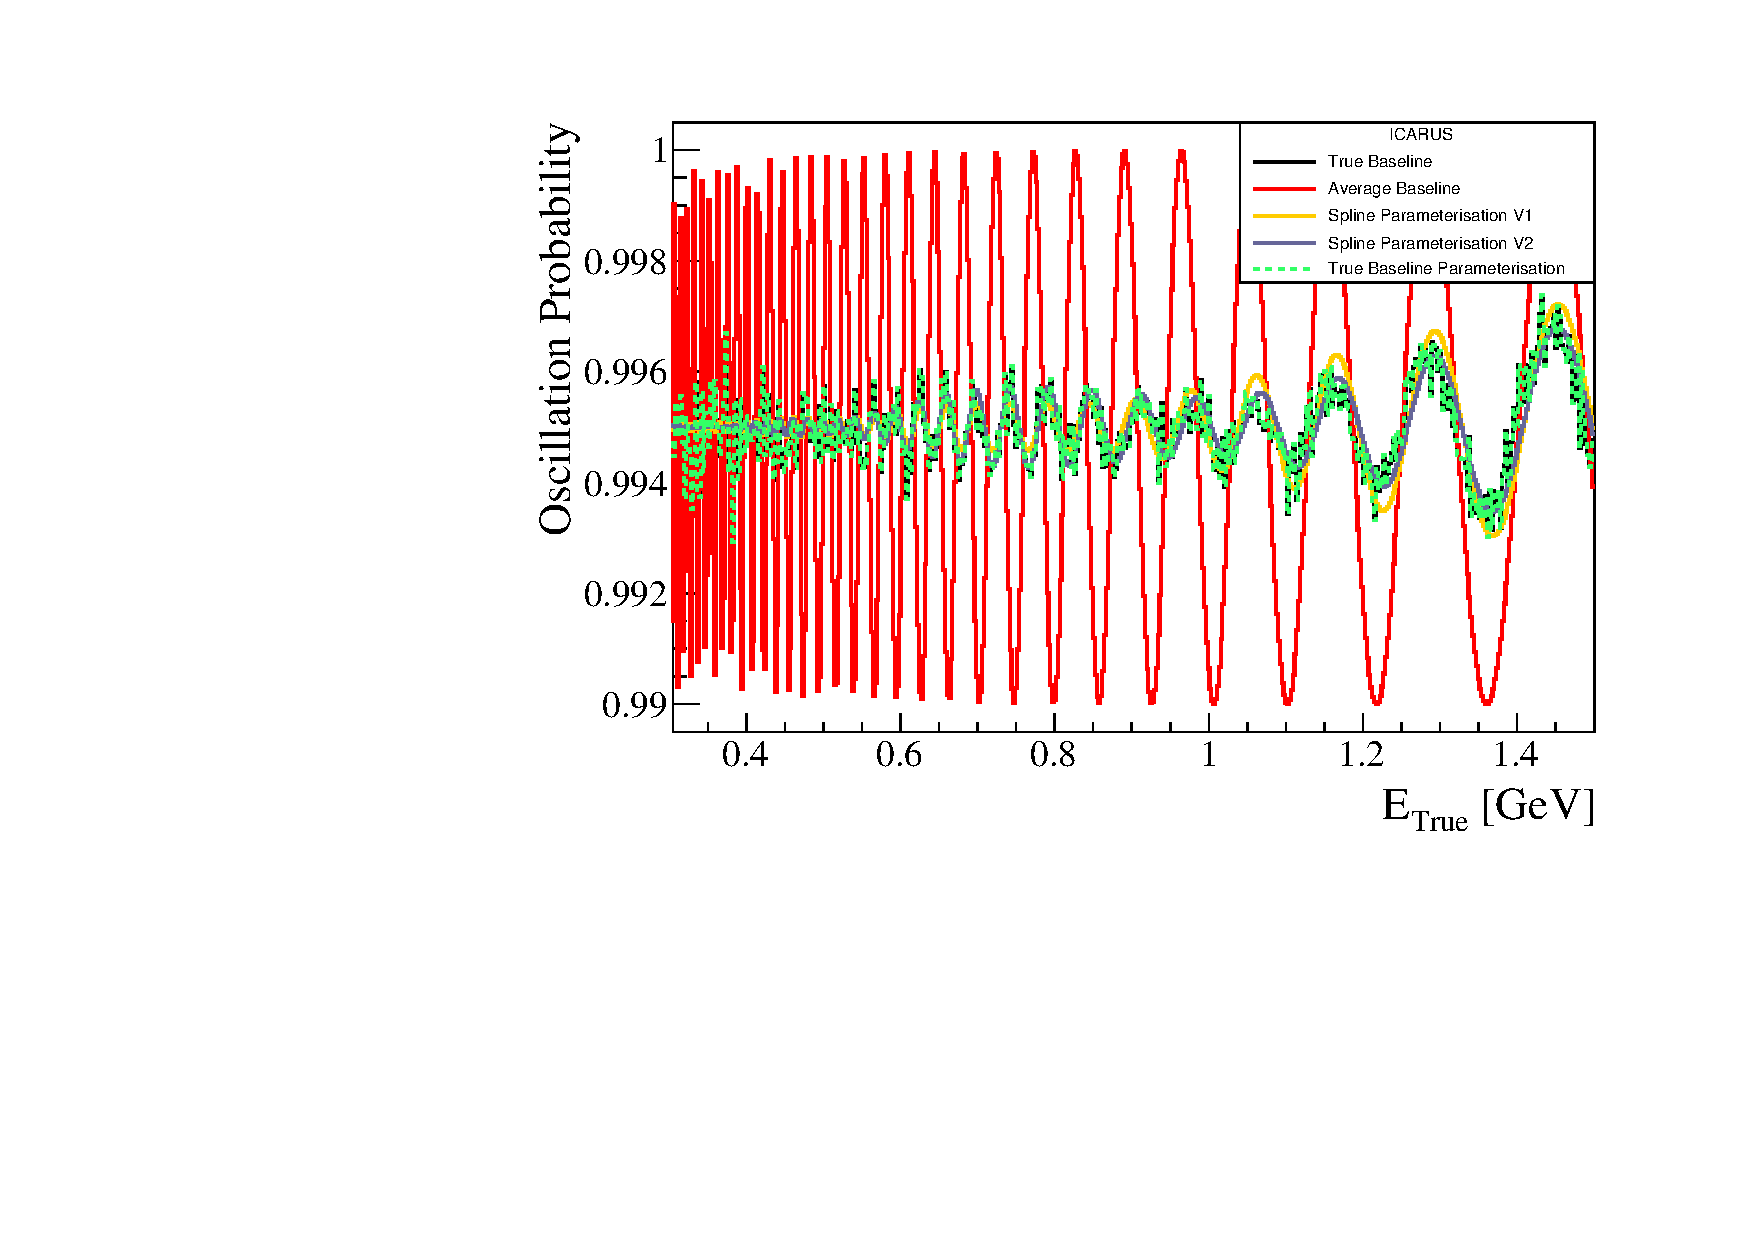
\includegraphics[width = 0.32\textwidth]{figures-chap5/osc_prob_icarus.pdf}
    \caption{The oscillation probability as a function of true neutrino energy for the \numu disappearance sample with oscillation parameters $sin^22\theta_{\mu\mu} = 0.01$ and $\Delta m^2_{41} = 50$ eV$^2$ in each \gls{sbn} detector. The results from using each baseline parametrisation are shown.}
    \label{fig:baseline_osc_probability}
\end{figure}

\subsection{Binning}\label{sec:binning}

The $\nu_\mu$ edge-to-edge binning has 21 bins in reconstructed neutrino energy which are bounded as follows:
\begin{itemize}
    \item 1 bin from 0.0-0.2 GeV,
    \item 2 0.1-GeV bins from 0.2-0.4 GeV,
    \item 12 0.05-GeV bins from 0.4-1.0 GeV,
    \item 2 0.25-GeV bins from 1.0-1.5 GeV,
    \item 3 0.5-GeV bins from 1.5-3.0 GeV and
    \item 1 bin from 3.0-10.0 GeV.
\end{itemize}

The $\nu_\mu$ edge-to-edge binning has 22 bins in true neutrino energy which are bounded as follows:
\begin{itemize}
    \item 1 bin from 0.00-0.30 GeV,
    \item 3 0.10-GeV bins from 0.30-0.60 GeV,
    \item 12 0.05-GeV bins from 0.60-1.20 GeV,
    \item 1 bin from 1.20-1.50 GeV,
    \item 3 0.50-GeV bins from 1.50-3.00 GeV,
    \item 1 bin from 3.00-5.00 GeV and
    \item 1 bin from 5.00-10.00 GeV.
\end{itemize}

The $\nu_e$ edge-to-edge binning has 12 bins in reconstructed neutrino energy which are bounded as follows:
\begin{itemize}
    \item 1 0.35-GeV bin from 0.00-0.35 GeV,
    \item 5 0.15-GeV bins from 0.35-1.10 GeV,
    \item 2 0.20-GeV bins from 1.10-1.50 GeV,
    \item 2 0.25-GeV bins from 1.50-2.00 GeV,
    \item 1 bin from 2.00-3.00 GeV and
    \item 1 bin from 3.00-10.00 GeV.
\end{itemize}

The $\nu_e$ edge-to-edge binning has 33 bins in true neutrino energy which are bounded as follows:
\begin{itemize}
    \item 2 0.25-GeV bin from 0.00-0.50 GeV,
    \item 15 0.05-GeV bins from 0.50-1.25 GeV,
    \item 15 0.25-GeV bins from 1.25-5.00 GeV and
    \item 1 bin from 5.00-10.00 GeV.
\end{itemize}

